%% FEUP THESIS STYLE for LaTeX2e
%% how to use feupteses for MIEIC dissertations
%%
%% FEUP, JCL & JCF,  Wed Oct  4 16:32:24 2017
%%
%% PLEASE send improvements to jlopes at fe.up.pt and to jcf at fe.up.pt
%%

%%========================================
%% Commands: pdflatex thesis
%%           bibtex thesis
%%           makeindex thesis (only if creating an index) 
%%           pdflatex thesis
%% Alternative:
%%          latexmk -pdf thesis.tex
%%========================================

\documentclass[11pt,a4paper,twoside,openright]{report}
\usepackage[utf8]{inputenc}
%\usepackage[latin1]{inputenc}

%%%%%%% English version 

%% MIEIC options
\usepackage[mieic]{feupteses}                  % work version
%\usepackage[mieic,juri]{feupteses}             % juri verrion
%\usepackage[mieic,final]{feupteses}            % final version

%% Additional options for feupteses.sty: 
%% - portugues: titles, etc in portuguese
%% - onpaper: links are not shown (for paper versions)
%% - backrefs: include back references from bibliography to citation place

%%%%%%% Portuguese version

%\usepackage[mieic,portugues]{feupteses}        % work version
%\usepackage[mieic,portugues,juri]{feupteses}   % juri version
%\usepackage[mieic,portugues,final]{feupteses}  % final version

%% Uncomment the next lines if side by side graphics used
%\usepackage[lofdepth,lotdepth]{subfig}
%\usepackage{graphicx}
%\usepackage{float}

\usepackage{url}
\usepackage{threeparttable}
\usepackage{adjustbox}

%% Include color package
\usepackage{color}
\definecolor{cloudwhite}{cmyk}{0,0,0,0.025}

%% Include source-code listings package
\usepackage{listings}
\lstset{ %
 language=C,                        % choose the language of the code
 basicstyle=\footnotesize\ttfamily,
 keywordstyle=\bfseries,
 numbers=left,                      % where to put the line-numbers
 numberstyle=\scriptsize\texttt,    % the size of the fonts that are used for the line-numbers
 stepnumber=1,                      % the step between two line-numbers. If it's 1 each line will be numbered
 numbersep=8pt,                     % how far the line-numbers are from the code
 frame=tb,
 float=htb,
 aboveskip=8mm,
 belowskip=4mm,
 backgroundcolor=\color{cloudwhite},
 showspaces=false,                  % show spaces adding particular underscores
 showstringspaces=false,            % underline spaces within strings
 showtabs=false,                    % show tabs within strings adding particular underscores
 tabsize=2,	                    % sets default tabsize to 2 spaces
 captionpos=b,                      % sets the caption-position to bottom
 breaklines=true,                   % sets automatic line breaking
 breakatwhitespace=false,           % sets if automatic breaks should only happen at whitespace
 escapeinside={\%*}{*)},            % if you want to add a comment within your code
 morekeywords={*,var,template,new}  % if you want to add more keywords to the set
}

%% Uncomment to create an index (at the end of the document)
%\makeindex

%% Path to the figures directory
%% TIP: use folder ``figures'' to keep all your figures
\graphicspath{{figures/}}

%%----------------------------------------
%% TIP: if you want to define more macros, use an external file to keep them
%some macro definitions

\RequirePackage{ifthen}

% format
\newcommand{\class}[1]{{\normalfont\slshape #1\/}}

% entities
\newcommand{\Feup}{Faculdade de Engenharia da Universidade do Porto}

\newcommand{\svg}{\class{SVG}}
\newcommand{\scada}{\class{SCADA}}
\newcommand{\scadadms}{\class{SCADA/DMS}}

\newcommand{\ie}{\emph{i}.\emph{e}., }
\newcommand{\eg}{\emph{e}.\emph{g}., }
\newcommand{\etal}{\emph{et al}. }
\newcommand{\cf}{\emph{cf}. }

\newcommand{\asidewaystable}[6]{
  \begin{sidewaystable}
  	\centering
  	\begin{tabularx}{\textwidth}{#1}
      \toprule
      #2
      \midrule
      \tablecontent{#3}
      \bottomrule
    \end{tabularx}
  	\caption[#6]{#5} \label{#4}
  \end{sidewaystable}
}

% Imported macros from Diogo

\RequirePackage{ifthen}

%%
%% Reference shorthands.
%%

\newcounter{cPage}
\newcommand\optref[1]{%
 \refstepcounter{cPage}\label{current\thecPage}%
 \ifthenelse{\equal{\pageref{#1}}{\pageref{current\thecPage}}}%
  {}{~(p.~\pageref{#1})}%
}

\newcommand\optrefparens[1]{%
 \refstepcounter{cPage}\label{current\thecPage}%
 \ifthenelse{\equal{\pageref{#1}}{\pageref{current\thecPage}}}%
  {}{,~p.~\pageref{#1}}%
}

\newcommand\coderef[1]{Source~\ref{#1}\optref{#1}}
\newcommand\figureref[1]{Figure~\ref{#1}\optref{#1}}
\newcommand\seefigureref[1]{(\emph{cf.} Figure~\ref{#1}\optrefparens{#1})}
\newcommand\tableref[1]{Table~\ref{#1}\optref{#1}}
\newcommand\chapterref[1]{Chapter~\ref{#1}\optref{#1}}
\newcommand\seechapterref[1]{(\emph{cf.} Chapter~\ref{#1}\optrefparens{#1})}
\newcommand\sectionref[1]{Section~\ref{#1}\optref{#1}}
\newcommand\seesectionref[1]{Section~\ref{#1}\optrefparens{#1}}
\newcommand\sectionintroref[1]{Section~\ref{#1}}

\newcommand\appendixref[1]{Appendix~\ref{#1}\optref{#1}}

% MiniTOC
\usepackage[tight]{minitoc}
\setcounter{minitocdepth}{1}
\renewcommand{\mtctitle}{}
\renewcommand{\kernafterminitoc}{\vspace{0.2cm}}
\renewcommand{\mtcoffset}{-0.3cm}

%%
%% Hyphenization
%%

\RequirePackage[english=usenglishmax]{hyphsubst}

%%
%% Page layout
%%

\raggedbottom

% No orphans
\clubpenalty = 500
\widowpenalty = 1000
% \checkandfixthelayout

%%
%% Line breaking
%%

\RequirePackage[final=true,step=1]{microtype}
\RequirePackage{ragged2e}

%%----------------------------------------

%%========================================
%% Start of document
%%========================================
\begin{document}

%%----------------------------------------
%% Information about the work
%%----------------------------------------
\title{Decentralized Orchestration of IoT in End-user Programming Environments}
\author{Ana Margarida Oliveira Pinheiro da Silva}

%% Uncomment next line for date of submission
%\thesisdate{July 31, 2008}

%%Uncomment next line for copyright text if used
%\copyrightnotice{Name of the Author, 2008}

\supervisor{Supervisor}{Hugo Sereno Ferreira}

%% Uncomment next line if necessary
\supervisor{Second Supervisor}{André Restivo}

%% Uncomment committee stuff in the final version 
%\committeetext{Approved in oral examination by the committee:}
%\committeemember{Chair}{Prof.\ Name of the President}
%\committeemember{External Examiner}{Prof.\  Name of the Examiner}
%\committeemember{Supervisor}{Prof.\ Name of the Supervisor}

%\committeetext{Aprovado em provas públicas pelo Júri:}
%\committeemember{Presidente}{Prof.\ Nome do presidente do júri}
%\committeemember{Arguente}{Prof.\ Nome do arguente do júri}
%\committeemember{Vogal}{Prof.\ Nome do vogal do júri}

%% Specify cover logo (in folder ``figures'')
\logo{uporto-feup.pdf}

%% Uncomment next line for additional text below the author's name (front page)
%\additionalfronttext{Preparação da Dissertação}

%%----------------------------------------
%% Preliminary materials
%%----------------------------------------

% remove unnecssary \include{} commands
\begin{Prolog}
  \chapter*{Abstract}

The Internet-of-Things (IoT) is an ever growing network of devices connected to the Internet. Such devices are heterogeneous in their protocols and computation capabilities. With the rising computation and connectivity capabilities of these devices, the possibilities of their use in IoT systems increases. Concepts like smart cities are the current pinnacle of the use of these systems, which will involve a big amount of different devices in different conditions.

There are several tools for building complex IoT systems; some of these tools have different levels of expertise required and employ different architectures. One of the most popular is Node-RED. It provides users with a visual data flow architecture, with the side effect of making it accessible for a non-developer as well.

Most of these mainstream tools employ centralized methods of computation where a main component --- usually hosted in the cloud --- executes most of the computation on data provided by edge devices, \emph{e.g.} sensors and gateways. There are multiple consequences to this approach: (a)~edge computation capabilities are being neglected, (b)~it introduces a single point of failure, and (c)~local data is transferred across boundaries (private, technological, political...) either without need, or even in violation of legal constraints. Particularly, the principle of Local-First --- \emph{i.e.}, data and logic should reside locally, independent of third-party services faults and errors --- is blatantly ignored.

Previous works in the domain of visual programming attempt to mitigate some of these consequences, going as far as to propose solutions to decentralize flows and their execution in fog/edge devices. But they mostly require that the decomposition and partitioning effort to be manually specified by the developer when building the system, limiting dynamic adaptation of the system to failures or appearance of devices.

In this work we propose a method for extending Node-RED to allow the automatic decomposition and partitioning of the system towards higher decentralization. With this in mind, we implemented custom firmware for exposing the resources of the available devices, as well as new \textit{nodes} and modification in Node-RED that allow orchestration of tasks. This firmware is responsible for low-level management of health and capabilities, as well as executing MicroPython scripts on demand. Node-RED was modified to take advantage of this firmware by (1) implementing a device registry that allows devices to announce themselves, (2) generating MicroPython code from \textit{flow} and \textit{nodes} and (3) assigning \textit{nodes} to devices based on pre-specified properties and priorities. Likewise, a mechanism was developed to automatically detect abnormal run-time conditions, providing dynamic self-adaptation.

Our solution was tested by implementing home automation scenarios, where several experiments were made with the use of both virtual and physical devices. Several metrics were measured to allow understanding the impact on the resiliency, efficiency and elasticity of the system. With this data, we were able to conclude that our approach scales in terms of number of devices and is more robust. We further identified remaining open challenges to be tackled in the future.

\vspace*{10mm}\noindent

\textbf{Keywords}: Internet-of-Things, Orchestration, Visual Programming, Distributed Systems, Real-Time, Embedded

% \ccsdesc[500]{Computer systems organization~Embedded systems}
% \ccsdesc[300]{Computer systems organization~Distributed architectures}
% \ccsdesc[100]{Computer systems organization~Reliability}
% \ccsdesc[300]{Software and its engineering~Embedded software}
% \ccsdesc[100]{Software and its engineering~Integrated and visual development environments}

\chapter*{Resumo}

A Internet-of-Things (IoT) é uma rede de dispositivos conectados à Internet em constante crescimento. Estes dispositivos são heterogéneos nos seus protocolos e capacidades de computação. Com o crescimento das capacidades de computação e conectividade destes dispositivos, as possibilidades do seu uso em sistemas IoT aumentaram. Conceitos como Cidades Inteligientes são o pináculo do uso destes sistemas, que envolverão um grande número de dispositivos diferentes.

Existem várias ferramentas para construir sistemas IoT; algumas destas ferramentas requerem diferentes níveis de perícia e usam diferentes arquiteturas. Uma das ferramentas mais populares é Node-RED, que permite aos utilizadores construir sistemas usando uma arquitetura visual de \emph{data flow}, tornando o processo mais fácil para um não programador.

No entanto, a maioria das ferramentas convencionais usam métodos centralizados de computação, onde um componente principal - normalmente alocado na \emph{cloud} - executa a maioria da computação nos dados provenientes dos dispositivos \emph{edge}, \emph{e.g.} sensores e \emph{gateways}. Esta abordagem tem diversas consequências: (a) capacidades de computação de dispositivos \emph{edge} estão a ser negligenciadas, (b) introduz um único ponto de falha, e (c) data local é transferida através de limites (privados, tecnológicos, políticos...) sem necessidade ou violando restrições legais. Especificamente, o princípio de \emph{Local-First} - \emph{i.e.}, dados e lógica devem residir localmente, independentemente de falhas e erros de serviços terceiros - é totalmente ignorado.

Trabalhos feitos no domínio de programação visual tentam mitigar algumas destas consequências, propondo uma solução que consiste na descentralização de \emph{flows} e a sua execução em dispositivos de \emph{fog} e \emph{edge}. Atualmente, para obter a este tipo de descentralização é necessário que o esforço de decomposição seja manualmente efetuado pelo programador na construção do sistema, limitando a adaptação dinâmica do sistema a falhas e aparecimento de dispositivos.

Neste documento propomos a extensão da ferramenta Node-RED para permitir a decomposição e partição automática do sistema para obter uma maior descentralização. Com isto em mente, implementámos \textit{firmware} específico que expõe os recursos dos dispositivos disponíveis, assim como novos nós e modificações no Node-RED que permitem a orquestração de tarefas. Este \textit{firmware} é responsável pela gestão do estado e capacidades do dispositivo, assim como a execução de código MicroPython sob demanda. Node-RED foi alterado com (1) uma implementação de um registo de dispositivos que permite que estes se anunciem, (2) geração de código MicroPython a partir de \textit{flows} e nós e (3) alocamento de nós a dispositivos baseado em propriedades e prioridades pré-definidas. Para além disto, foi desenvolvido um mecanismo que deteta automaticamente condições anormais dos dispositivos em \emph{run-time}, levando o sistema a adaptar-se.

Para testar a nossa solução foram implementados cenários de \textit{home automation}, onde diversas experiências foram feitas usando dispositivos virtuais e físicos. Foram medidas várias métricas para permitir perceber o impacto na resiliência, eficiência e elasticidade do sistema. Com estes dados, pudemos concluir que a solução desenvolvida escala no número de dispositivos e é robusta. Foram identificados vários desafios por resolver, que ficam em aberto para trabalho futuro.

\vspace*{10mm}\noindent

\textbf{Keywords}: Internet-of-Things, Orchestration, Visual Programming, Distributed Systems, Real-Time, Embedded
  % the abstract
  \chapter*{Acknowledgements}
%\chapter*{Agradecimentos}

There is a big number of people that made it possible for me to finish my \textit{Master's Degree} and this dissertation.

First of all, I would like to thank my supervisors Hugo Sereno Ferreira and André Restivo, who guided me through the dissertation while supplying knowledge and insights that improved my knowledge and work. I also appreciated the electronics lessons given which might have created my new hobby. I would also like to thank João Pedro Dias for the insights and suggestions given, which greatly improved the final work.

I would like to thank my friends, who supported me through all this time and provided the best quality jokes for me to laugh about. A special thanks to my \textit{dissertation budies} from \textit{IoTices}, who always listened to my ramblings and provided support and companionship. 

To Pedro Reis, my boyfriend, for putting up with my many moods, motivating me, and reminding me when I needed to rest.

Lastly, a huge thank you to my parents and brother, who supported me through all my life and pushed me to be the best I can be. 

\vspace{10mm}
\flushleft{Ana Margarida Silva}
   % the acknowledgments
  \cleardoublepage
\thispagestyle{plain}

\vspace*{8cm}

\begin{flushright}
  \textsl{``While it is always best to believe in oneself, \\
  a little help from other can be a great blessing.''}\\
\vspace*{1.5cm}
    Uncle Iroh
\end{flushright}
     % initial quotation if desired
  \cleardoublepage
  \pdfbookmark[0]{Table of Contents}{contents}
  \tableofcontents
  \cleardoublepage
  \pdfbookmark[0]{List of Figures}{figures}
  \listoffigures
  \cleardoublepage
  \pdfbookmark[0]{List of Tables}{tables}
  \listoftables
  \chapter*{Abbreviations}
\chaptermark{ABBREVIATIONS}
%\chapter*{Acrónimos}
%\chaptermark{ACRONIMOS}


\begin{flushleft}
\begin{tabular}{l p{0.8\linewidth}}
API      & Application Programming Interface\\
CPSCN    & Cyber Physical Social Computing and Networking\\
CPU      & Central Processing Unit\\
IEC      & International Electrotechnical Commission\\
ISO      & Internation Organization for Standardization\\
IFTTT    & \textit{If This Then That}\\
IoT      & Internet-of-Things\\
JSON     & JavaScript Object Notation\\
MQTT     & Message Queuing Telemetry Transport\\
MTTR     & Mean Time To Recover\\
QoS      & Quality of Service\\
RaaS     & Robot as a Servive\\
IIoT     & Internet of Intelligent Things\\
REST     & Representational State Transfer\\
VPL      & Visual Programming Language\\
WWW      & \textit{World Wide Web}\\
\end{tabular}
\end{flushleft}

  % the list of abbreviations used
\end{Prolog}

%%----------------------------------------
%% Body
%%----------------------------------------
\StartBody

%% TIP: use a separate file for each chapter
\chapter{Introduction} \label{chap:intro} \minitoc

\section*{}

This chapter introduces the motivation and scope of this project, as well as the problems it aims to solve. Section \ref{sec:context} details the context of this project in the area it is based on. Section \ref{sec:problem_definition} defines the problem we aim to solve. Then, Section \ref{sec:motivation} explains the reason why this work and the area it belongs to is important and the goals of this dissertation are described in Section \ref{sec:goals}. Finally, the Section \ref{sec:document structure} describes the structure of this document and what content it contains.

\section{Context} \label{sec:context}

The Internet-of-Things(IoT) paradigm states that all devices, independently of their capabilities, are connected to the Internet and allow for the transfer, integration and analytic of data generated by them \cite{IoT_principles_and_paradigms}. This paradigm has several characteristics, such as the heterogeneity and high distribution of devices as well as their increasing connectivity and computational capabilities \cite{SoS}. All these factors allow for a great level of applicability, enabling the realization of systems for management of cities, health services and industries \cite{6851114}.

The interest in Internet-of-Things has been growing massively, following the rising of connected devices along these past years. According to Siemens, in 2020 there will be around 26 billion physical devices connected to the Internet and in 2025 the predictions are pointing at 75 billion \cite{tanweer}. Although this allows for more opportunities, it is important to note that these devices are very different in their hardware and capabilities, which causes several problems in terms of development the systems, as well as their scalability, maintainability and security. 

Visual Programming Languages (VPLs) allow the user to communicate with the system by using and arranging visual elements that can be translated into code \cite{vpl-book}. It provides the user with an intuitive and straightforward interface for coding at the possible cost of loosing functionality. There are several programming languages with different focuses, such as education, video game development, 3D building, system design and even Internet-of-Things \cite{survey_vpl_iot}. Node-RED\footnote{https://nodered.org/} is one of the most famous open source visual programming tool, originally developed by IBM’s Emerging Technology Services team and now a part of the JS Foundation, which provides an environment for users to develop their own Internet-of-Things systems.

Non-functional attributes in a system are very important, specially attributes such as resiliency, fault-tolerance and self-healing in Internet-of-Things systems. All these attributes mean that when an error or problem occurs, the system can adapt and overcome them in a dynamic and automatic way.

Node-RED, mentioned above, is a centralized system, as well as most of the visual programming environments applied to IoT. A centralized architecture has a central instance that executes all computational tasks on the data provided by the other devices in the network. On the other hand, in a decentralized architecture the central instance, if it exists, partitions the computational tasks in independent blocks that can be executed by other devices. In IoT, these decentralized architectures are mentioned in Fog and Edge computing.

\section{Problem Definition} \label{sec:problem_definition}

Most mainstream visual programming tools focused on Internet-of-Things, Node-RED included, have a centralized approach, where a main component executes most of the computation on data provided by edge devices, e.g. sensors and gateways. There are several consequences to this approach: (a)~computation capabilities of the edge devices are being ignored, (b)~it introduces a single point of failure, and (c)~local data is being transferred across boundaries (private, technological, political...) either without need, or even in violation of legal constraints. The principle of Local-First \cite{localfist} - i.e, data and logic should reside locally, independent of third-party services faults and errors - and NoCloud \cite{nocloud} - i.e, on-device and local computation should be prioritized over cloud service computation - is being ignored. 

Besides being a single point of failure, centralized systems can be less efficient than decentralized ones and in this context it might be the case, since there are computation capabilities that aren't being taken advantage of.

Chapter \ref{chap:problem_statement} expands on the problem definition, explaining it in bigger detail, defining its scope, desiderata, use cases and research questions.

\section{Motivation} \label{sec:motivation}

Internet-of-Things is a rapid growing concept that is being applied to several areas, such as home automation, industry, health, city management and many others. Given the number of existing systems with different protocols and architectures, it becomes difficult for a user to build a system that is in accordance to standards \cite{standard-iot}. 

With the appearance of visual programming languages focused in IoT, more specifically Node-RED, users can build their own systems in an easier and streamlined way, removing the overhead of learning advanced programming concepts and protocols. These tools must be resilient, in order to withstand flaws and non-availability of devices as well as failure in the network. However, the majority of these tools are centralized, including Node-RED, and this type of architecture hinders the resiliency of the system. Given the existence of only one unit that executes most or all the processing of data, if this device fails, the system becomes non functional. A possible solution would be increasing the redundancy of the system, creating more than one instances of the main unit. However, this approach has several costs, not only monetary but also in the increase of complexity.

\section{Goals} \label{sec:goals}

The main goal of this dissertation is to leverage the computation capabilities of the devices in the network, increasing efficiency, fault-tolerance, resiliency and scalability in an Internet-of-Things system.

To achieve this goal, a prototype will be developed, extending or rewriting Node-RED, that enables IoT devices to communicate their "computational capabilities" back to the orchestrator. In its turn, the orchestrator is able to partition the computation and send "tasks" to the nodes, which are the devices in the network, leveraging their computation power and independence.

As a secondary goal, several other challenges will be tackled, viz: (i)~computational capabilities of the devices in the network, (ii)~detecting non-availability and using alternative computation resources, and (iii)~exploring different alternatives of leveraging current IoT devices, including using firmwares that allow the execution of programs written in Lua, Javascript, Python, etc., amongst others.

\section{Document Structure} \label{sec:document structure}

Chapter \ref{chap:background} introduces the background information and explanation about concepts necessary for the full understanding of this dissertation. Chapter \ref{chap:sota} describes the state of the art regarding the ecosystem of this project's scope, including a Systematic Literature Review on the state of the art of visual programming applied to the Internet-of-Things paradigm. Chapter \ref{chap:problem_statement} presents the problem this dissertation aims to solve, as well as the approach taken to solve it. Finally, Chapter \ref{chap:concl} concludes this dissertation with a reflection on the future contributions of this project.

%Chapter \ref{chap:concl} concludes the dissertation with a reflection on the success of the project by presenting the a summary of the contributions made and detailing the difficulties and future work.

%Chapter \ref{chap:solution} details how the solution was implemented and all the decisions and efforts taken to answer the problem statement mentioned before. Chapter \ref{chap:evaluation} analyzes the evaluation process and explains how the solution was validated 
\chapter{Background} \label{chap:background}

\section*{}

\minitoc \mtcskip \noindent
This chapter describes the necessary foundations regarding the Internet-of-Things context. \sectionintroref{sec:background_iot} describes the background of the Internet-of-Things paradigm and important concepts in that area, with a description of IoT architectures, including Fog and Edge, in \sectionintroref{sec:architectures}. Finally, \sectionintroref{sec:background_vpl} mentions visual programming languages, their uses as well as their benefits and drawbacks.

\section{Internet-of-Things}\label{sec:background_iot}

The Internet-of-Things paradigm is defined by the committee of the International Organization for Standardization and the International Electrotechnical Commission~\cite{ISOIEC} as:

\begin{quote}
    \emph{"An infrastructure of interconnected objects, people, systems and information resources together with intelligent services to allow them to process information of the physical and the virtual world and react."}
\end{quote}

\noindent
IoT systems are, mostly, networks of heterogeneous devices attempting to bridge the gap between people and their surroundings. According to Buuya~\cite{iot_future_direction}, the applications of IoT systems can be divided into four categories: (i)~\textit{Home}, at the scale of a few individuals or domestic scenarios, (ii)~\textit{Enterprise}, at the scale of a community or larger environments, (iii)~\textit{Utilities}, at a national or regional scale and (iv)~\textit{Mobile}, which is spread across domains due to its large scale in connectivity and scale. 

One might think that IoT only relates to machines and interactions between them. Most of the devices we use in our day-to-day --- \emph{e.g.}, mobile phones, security cameras, watches, coffee machines --- are computation capable of making moderately complex tasks and are continually generating and sending information. This incrementally translates towards the \emph{human-in-the-loop} concept, where humans and machines become part of a "symbiotic" relationship~\cite{human_in_the_loop_survey}.
 
\subsection{IoT architectures}\label{sec:architectures}

Internet-of-Things systems deal with big amounts of data from different sources and have to process it in an efficient and fast fashion~\cite{lin_survey}. Typical IoT systems are composed of three tiers~\cite{Yang2019}, which are:

\begin{description}
    \item[Cloud Tier] mostly composed of data centers and servers, normally running remotely. It is characterized by having high computation power and latency.
    \item[Fog Tier] composed of gateways and devices that are normally between the cloud servers and the edge devices. This tier has less latency than the cloud, more heterogeneity, and, typically, is more geographically distributed.
    \item[Edge Tier] composed of all the peripheral devices (\emph{e.g.}, sensors, embedded systems, light sources and air conditioners). These devices have several limitations in computational capabilities, but exhibit less latency since the data is processed in the same place it is captured.
\end{description}

Complementary to these tiers, we can also partition IoT systems into an Application Layer, a Network Layer, and a Perception Layer~\cite{iot_layers}. At first sight, these might seem compatible with the tiers mentioned above (in the same order); however, not all devices in each tier map to their respective layer. One example is a third-party service that provides readings, \eg Application Programming Interface (API) that provide temperature readings. It can be contained in the Perceptive Layer, but it is not included in the Edge Tier.

New paradigms of computing emerged related to each of these tiers. The majority of IoT systems use a Cloud Computing architecture~\cite{cisco}, taking advantage of centralized computing and storage. This approach poses some benefits, such as increased computational capabilities and storage, as well as easier maintenance. However, it also comes with several shortcomings such as (1)~higher latency, and~(2) higher usage of bandwidth, due to the need to send the data generated from the sensors back to the centralized unit(s)~\cite{connecting_fog_and_cloud}. Systems that only use cloud computing face several challenges~\cite{aazam2014cloud}, especially in real-time applications, which are sensitive to increased latency~\cite{latency_critical}. But with the increasing computation capabilities of edge devices and the requirement of reduced latency, two new paradigms appeared: Fog Computing and Edge Computing.

\subsubsection{Fog Computing}\label{sec:fog_computing}

The improvement of wireless technologies and the increasing computational power and reduced costs of lower-tier devices (\emph{i.e.}, fog and edge) allow the usage of these devices as computational resources in IoT systems. By not depending so much on the cloud tier, communication and resource sharing between devices can occur with lower latency and reduced amount of data transferred to the central instance. The central coordinator (on-premises or cloud-based), which in Cloud Computing was responsible for all the computation, now serves as an orchestrator of the communication between devices, occasionally providing necessary resources. This paradigm is called Fog Computing, where fog and edge devices are leveraged as computational entities, instead of merely sensors, actuators and gateways. It focuses on distributing data throughout the IoT system, from the cloud to the edge devices, making the system distributed and bringing computation closer to the perception tier~\cite{mobile_cloud}.

According to Buuya~\cite{IoT_principles_and_paradigms}, Fog Computing poses several advantages: (1)~reduction of network traffic by having edge devices filtering and analyzing the data generated and sending data to the cloud only if necessary, (2)~reduced communication distance by having the devices communicate between them without using the cloud as a middleman, (3)~low-latency by moving the processing closer to the data source rather than communicating all the data to the cloud for it to be processed, and (4)~scalability by reducing the burden on the cloud, which could be a bottleneck for the system.

\begin{figure}[h]
\centering
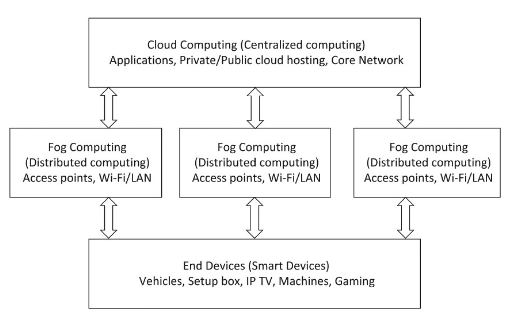
\includegraphics[width=0.8\textwidth]{fog_computing_architecture.png}
\caption[Fog Computing Architecture]{Fog Computing Architecture~\cite{IoT_principles_and_paradigms}}
\label{fig:fog_architecture}
\end{figure}

Despite all the advantages, Fog Computing has several challenges and difficulties. One of them is the management of resources and service allocation, responsible for deciding which tasks will be performed in the fog and where in the fog they will be allocated ~\cite{mukherjee}. The complexity is also more significant than Cloud Computing since it needs to work with heterogeneous devices with different capabilities.
       
\subsubsection{Edge Computing}\label{sec:edge_computing}

Edge Computing, also known as Mist Computing, is a distributed architecture that uses the devices' computational power to process the data they collect or generate. It takes advantage of the Edge tier, which contains the devices closer to the end-user, such as smartphones, TVs and sensors. The goal of this paradigm is to minimize the bandwidth and time response of IoT systems while leveraging the computational power of the devices in them. It reduces bandwidth usage by processing data instead of sending it to the cloud to be processed, which is also correlated to reduced latency since it does not wait for the server response. In addition to these advantages, and related to their cause, Edge Computing also prevents sensitive data from leaving the network, reducing data leakage and increasing security and privacy~\cite{edge_computing, edge_computing_2019}.

In this paradigm, each device serves both as a data producer and a data consumer. Since each device is constrained in terms of resources, this brings several challenges such as system reliability and energy constraints due to short battery life. Other issues consist of the lack of easy-to-use tools and frameworks to build cloud-edge systems, non-existent standards regarding the naming of edge devices and the lack of security edge devices have against outside threats such as hackers~\cite{promise_of_edge_computing}.

There is some confusion in the research community regarding the concepts of Fog and Edge computing. The publication from Iorga et al.~\cite{fog_edge_differences} was used to inspire the definitions of these terms. Edge Computing focuses on executing applications in constrained devices, without worrying about storage or state preservation. On the other hand, Fog Computing is hierarchical and includes devices with more capabilities, capable of control activities, storage, and orchestration.

\subsection{IoT development tools}\label{sec:iot_tools}

There are several tools that allow the development of IoT systems, with some of them being specific to certain domains and use-cases. \sectionref{sec:home_assistant} presents and IoT development tool focused on the home automation domain, where \sectionref{sec:device_hive} presents a more generic tool.

\subsubsection{Home Assistant}\label{sec:home_assistant}

Home Assistant~\cite{home_assistant} is an open-source home automation system that supports several mainstream IoT devices such as ESPs, Amazon Alexa, Google Assistant, and others. The configuration of the system is made with the use of a \textit{.yaml} file that is loaded by the system when it starts. This configuration file contains the integrations to be made and their respective configurations.

After creating the system, the user can interact with it by using a progressive web application. The interface, which consists of a dashboard, can be modified by the user to match its needs, with the addition of new panels or even the creation of new elements. It has integration with their Lovelace~\footnote{https://github.com/home-assistant/frontend/} front-end and React~\footnote{https://reactjs.org/}. An example of a Home Assistant dashboard can be seen in \figureref{fig:home_assistant}. 

\begin{figure}[h]
\centering
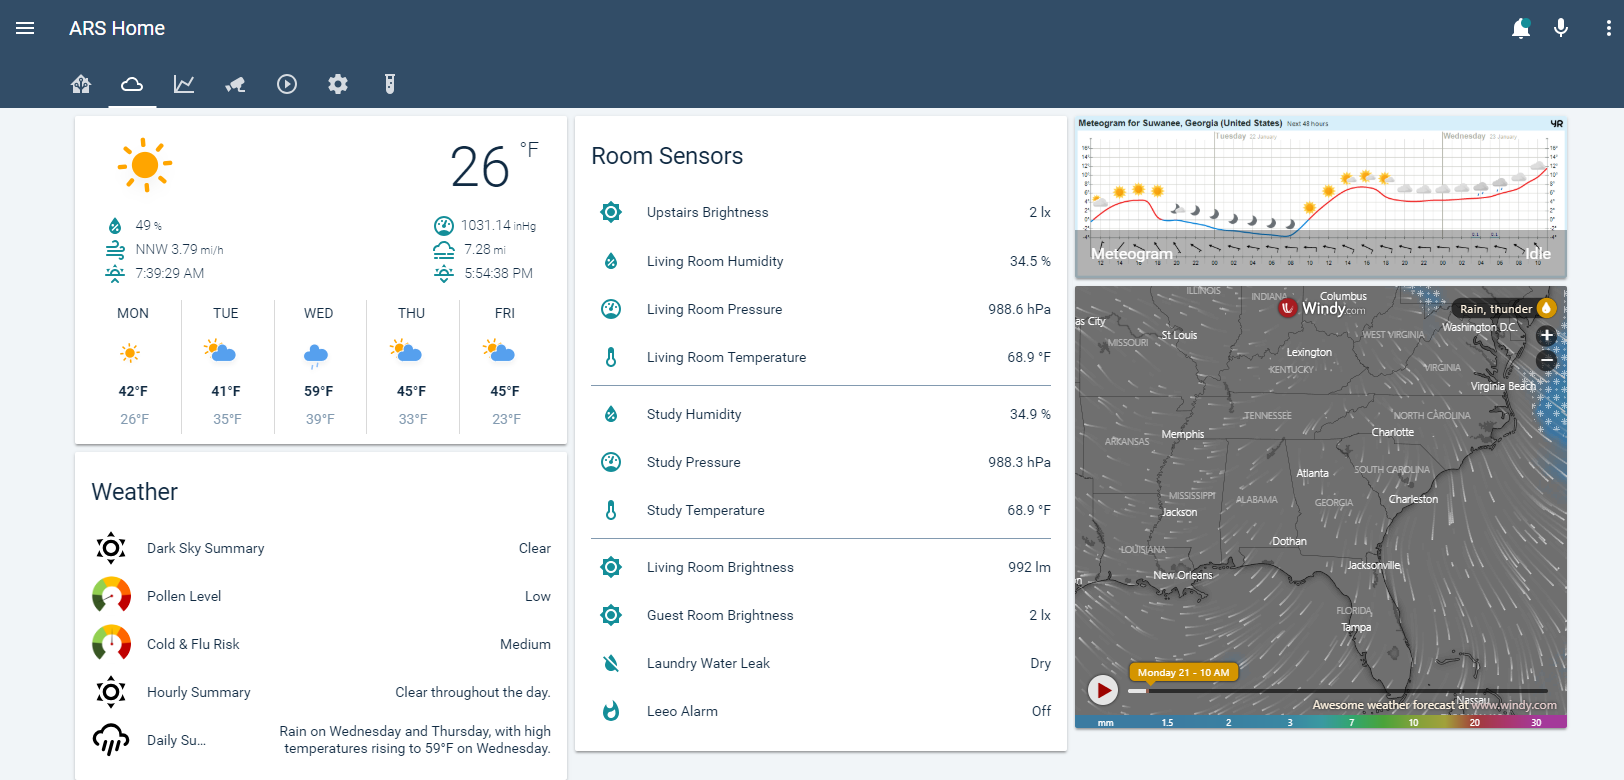
\includegraphics[width=1\textwidth]{home_assistant.png}
\caption[Example of a Home Assistant dashboard]{Example of a Home Assistant dashboard~\cite{homeassistant_image}}
\label{fig:home_assistant}
\end{figure}

The backend is made using Python3 and is composed of three modules: (1) the Home Control, responsible for collecting information and controlling the devices, (2) the Home Automation, responsible for triggering commands based on the user configuration, and (3) the Smart Home, for triggering commands based on previous interactions.

\subsubsection{Device Hive}\label{sec:device_hive}

Device Hive~\cite{device_hive} is an open-source IoT platform that supports multi-platform libraries for the development of IoT system in several domains (\eg home automation, smart energy, monitoring, remote control and others). It integrates with different types of devices, allowing modularity not only in the construction of client applications but also in the interfaces that connect with the devices. Device Hive is composed of three components: (1) the Auth service, responsible for the authorization and authentication of users and plugins, (2) the WebSocket Kafka Proxy, responsible for establishing communication between devices as well as allowing users to interact with plugins, and (3) the Plugin Management Service, that provides information about plugins, allows operations upon them and also allows the management of device operations.

Although the main core of the tool is a server that deals with all the devices and their data, it provides modules that can be integrated into the tool. They provide an Admin panel, which allows users to visually manage the connected devices and the installed plugins. It also integrates with Grafana~\footnote{https://grafana.com/} for data visualization. 

\section{Visual Programming Languages}\label{sec:background_vpl}

Having seen the characteristics and different ties of IoT, we will now address one of the most user-friendly ways of developing IoT systems.

Visual Programming, as defined by Shu~\cite{vpl_definition_shu}, consists of using meaningful graphical representations in the process of programming. We can consider Visual Programming Languages (VPLs) as a way of handling visual information and interaction with it, allowing the use of visual expressions for programming. According to Burnet and Baker~\cite{scaling_vpls}, visual programming languages are constructed to \emph{ "improve the programmer's ability to express program logic and to understand how the program works"}. There are several applications of visual programming languages in different areas, such as education, video game development, automation, multimedia, data warehousing, system management, and simulation, with this last area being the one with the most use cases~\cite{survey_vpl_iot}.

Visual programming languages exhibit several characteristics, such as a concrete and visual process and depiction of the program, immediate visual feedback, and usually require less knowledge of programming concepts~\cite{scaling_vpls}. VPLs can be categorized~\cite{vpls_survey} in the following way: 
\begin{description}
    \item[Purely Visual Languages], where the system is developed using only graphical elements and the subsequently debugging and execution is made in the same environment;
    \item[Hybrid text and visual systems], where the programs are created using graphical elements, but their execution is translated into a text language;
    \item[Programming-by-example systems], where a user uses graphical elements to teach the system;
    \item[Constraint-oriented systems], where the user translates physical entities into virtual objects and applies constraints to them, in order to simulate their behaviour in reality;
    \item[Form-based systems], which are based on the architecture and behaviour of spreadsheets.
\end{description}

Some of these categories can be simultaneously present in a single system, making them not mutually exclusive.

\subsection{Node-RED}\label{sec:node-red}

Node-RED~\cite{node_red} is a visual programming tool applied to the development of Internet-of-Things systems. It was first developed to manipulate and visualize mappings between Message Queuing Telemetry Transport (MQTT) topics in IBM's Emerging Technology Services group. It then expanded into a more general open-source tool, which is now part of the JS Foundation.

It is a web-based tool consisting of a run time built with the Node.js framework and a browser-based visual editor. This tool provides the end-user with a simple interface to connected devices and APIs, using a flow-programming approach~\cite{node_red}. Programs are called \emph{flows}, built with \emph{nodes} connected by wires. Each node corresponds to an action, such as input, output, data processing, etc.

The Node-RED interface has three components: (1)~Palette, (2)~Workspace and (3)~Sidebar. The Palette contains all the nodes installed and available to use, divided into categories. They can be used by dragging them into the workspace and additional features for each node are accessible by double-clicking them. The Workspace is where the flows are created and modified. It is possible to have several \emph{flows} and \emph{sub-flows} accessible with the use of tabs. Lastly, the Sidebar contains information about the nodes, the debug console, node configuration manager and the context data. \figureref{fig:node_red_window} showcases the visual interface of Node-RED and its elements.

\begin{figure}[h]
\centering
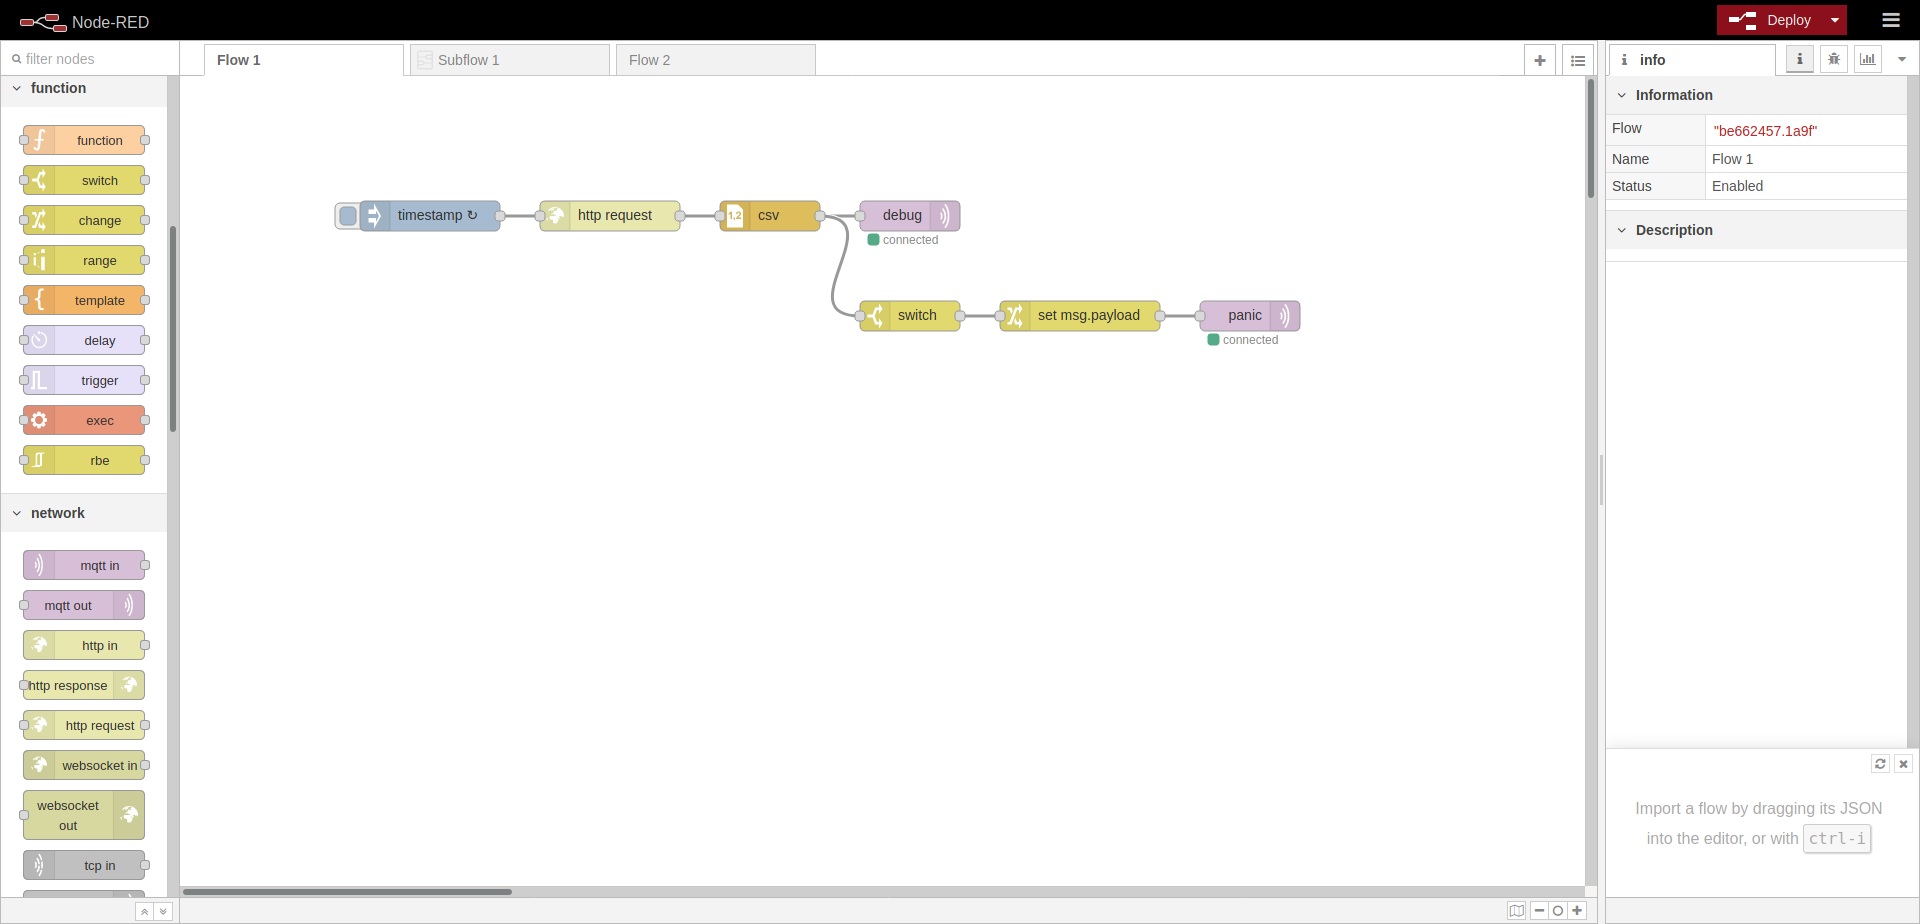
\includegraphics[width=1\textwidth]{node_red_window.png}
\caption{Node-RED environment}
\label{fig:node_red_window}
\end{figure}

One example of a \emph{flow} can be seen in \figureref{fig:node_red_example}, where a request is being made in intervals of 5 minutes to an HTTP URL that returns a CSV with the feed of significant earthquakes in the last 7 days. The data from the CSV is then printed to a MQTT topic and, if the magnitude is equal or bigger than 7, the message "PANIC!" is printed to other MQTT topic. 

\begin{figure}[!ht]
\centering
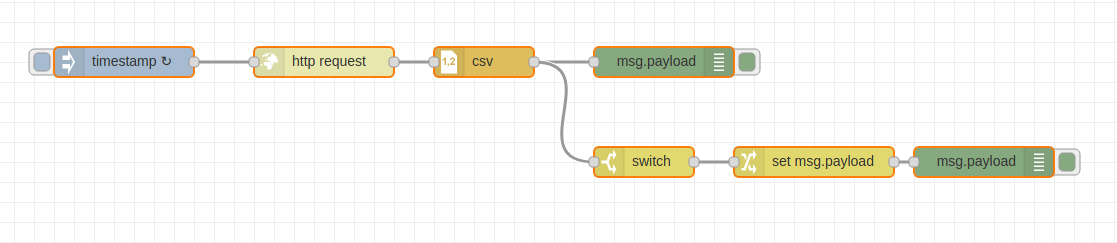
\includegraphics[width=1\textwidth]{node_red_example.png}
\caption{Example of a Node-RED flow}
\label{fig:node_red_example}
\end{figure}

Node-RED is modular, allowing the installation of community-made extensions, such as \textit{nodes}. These custom nodes extend from the base class \texttt{Node}, which implements an event based communication. Each node sends and receives messages, triggering events that execute each \textit{node}'s specific behaviour.

Being open-source, Node-RED takes advantage of a large community that contributes with new nodes and improvements to the tool. It is the most popular open-source visual programming tool for IoT, with more than 9,300 stars on Github.

\subsection{Godot}\label{sec:godot}

There are also other domains besides IoT where visual programming languages are being used. One example is the game engine Godot~\footnote{https://godotengine.org/} with its visual scripting. Godot is an open-source game engine that has recently increased in popularity, currently having 31,600 stars on GitHub~\footnote{https://github.com/godotengine/godot}. It offers several alternatives for its users to program their games, from using C++ to their own GDScript. However, to lower the barrier for a user to start using the engine, allowing people with no programming experience to easily understand the flow of logic, they developed a visual alternative --- visual scripting \seefigureref{fig:godot}.

\begin{figure}[!ht]
\centering
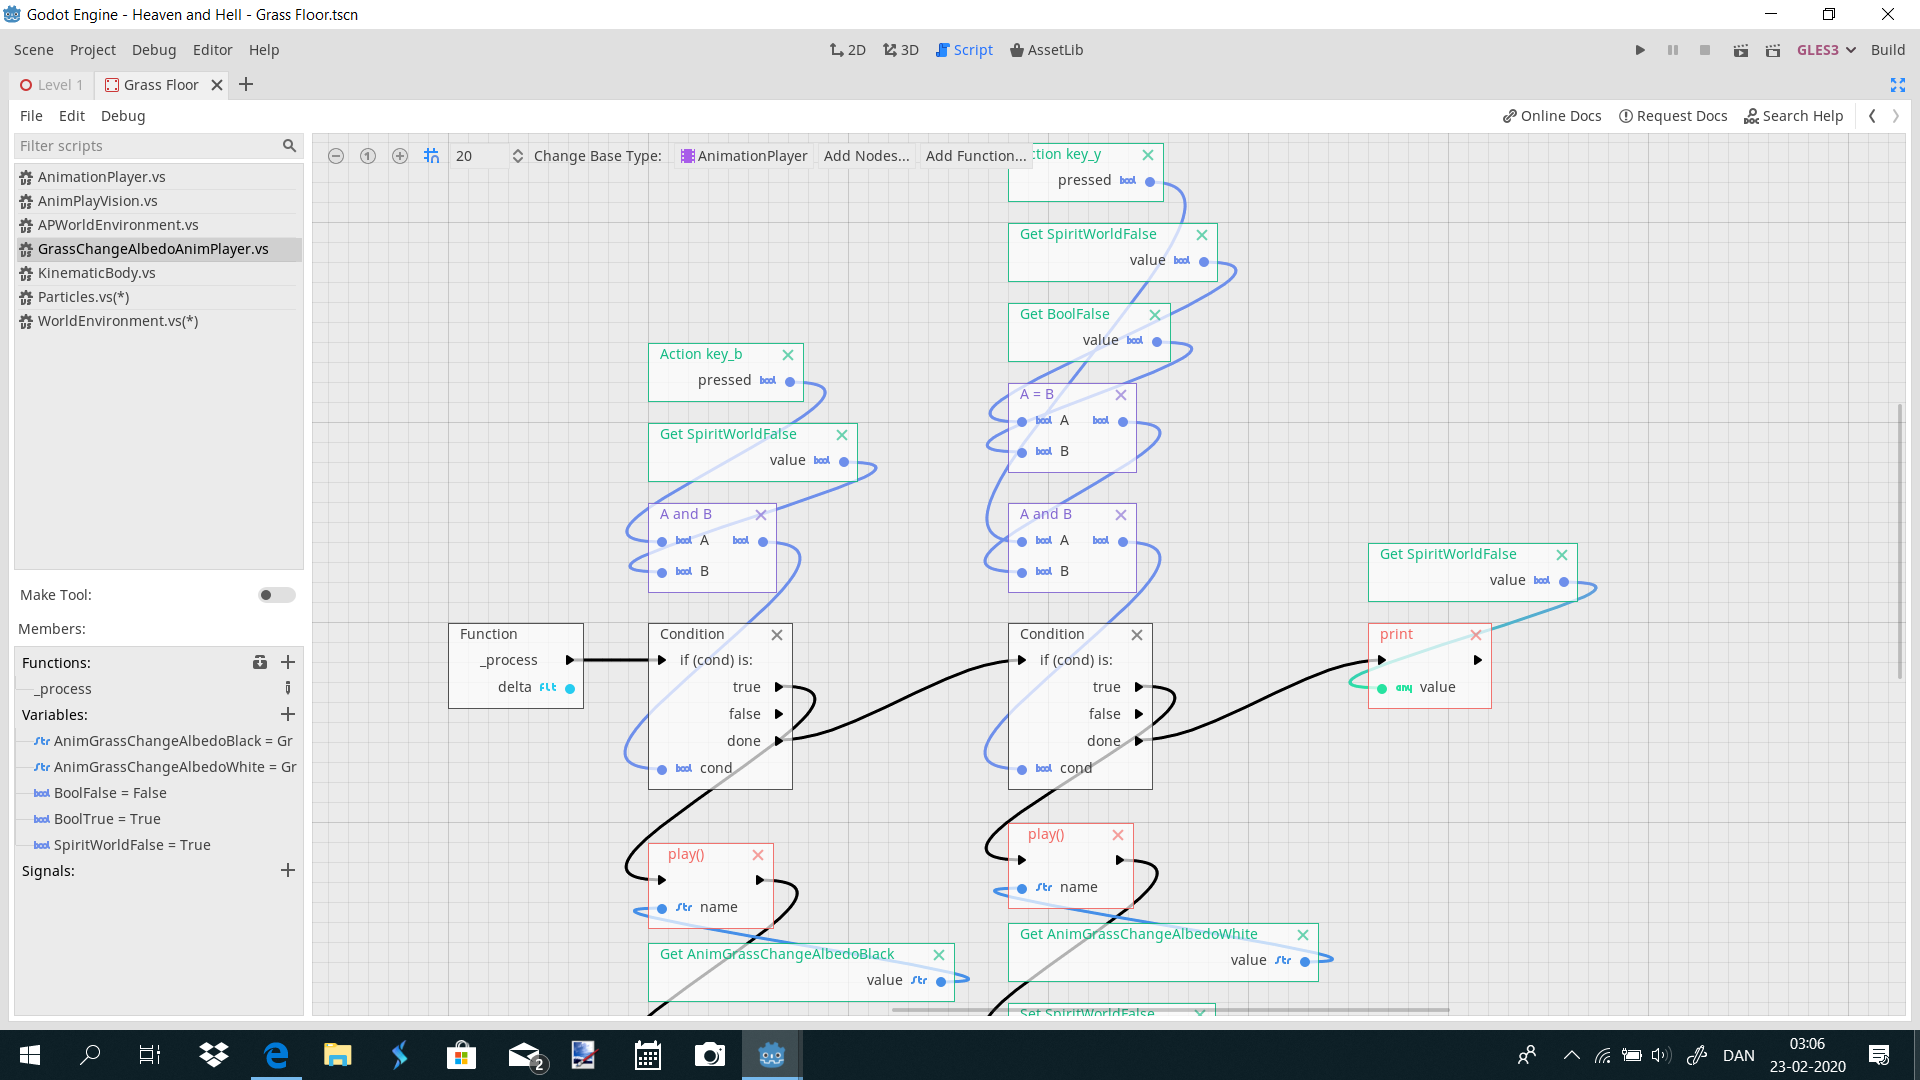
\includegraphics[width=1\textwidth]{godot_vpl.png}
\caption[Godot visual scripting]{Godot visual scripting~\cite{godot_image}}
\label{fig:godot}
\end{figure}

Each node corresponds to a function in a normal text script. Each node contains properties, ports and connections. Properties consist of arguments the function receives, as well as arguments globally accessible by the script. Ports and connections consist of inputs and outputs it can receive, either from other nodes or signals emitted during the events of the game.

Although most features are implemented in this visual alternative, it does not substitute programming with code, since visual scripting takes more time to develop code and it hinders project scalability.

\subsection{Blender}\label{sec:blender}

Blender~\footnote{https://www.blender.org/} is an open-source 3D creation suite that supports that entirety of the 3D pipeline. It is open to the community, with its source code being under the GPL license. It contains a visual programming editor, called Node Editor, which works with 3 types of nodes: (i) material, (ii) composite and (iii) texture nodes. \figureref{fig:blender} contains an example of a composition.

\begin{figure}[!ht]
\centering
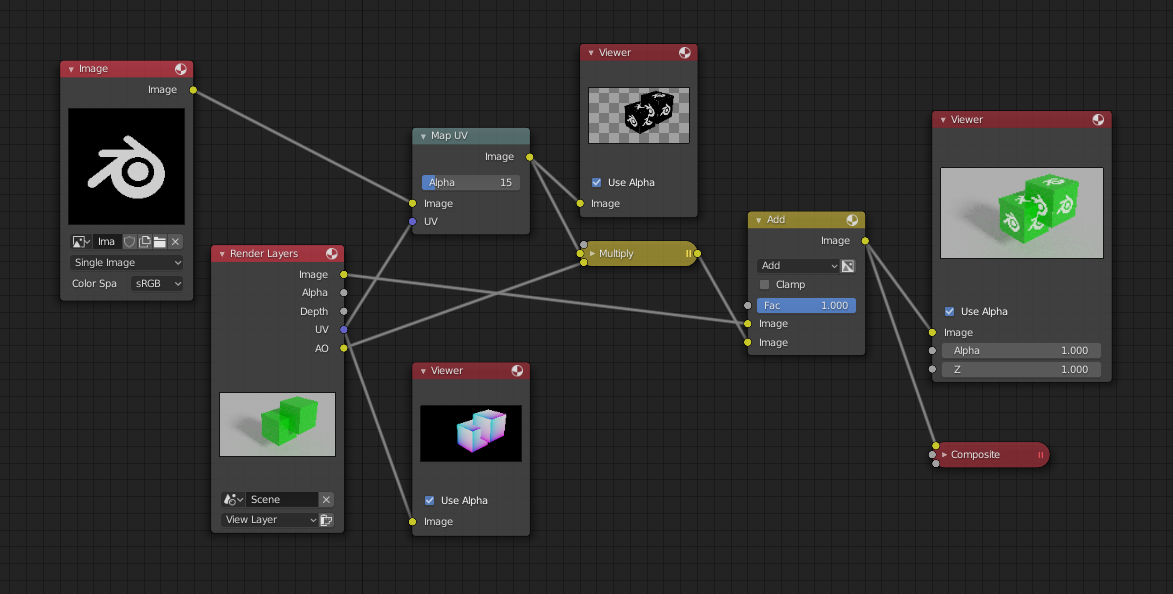
\includegraphics[width=1\textwidth]{blender_image.png}
\caption[Blender composition node editor]{Blender composition node editor~\cite{blender_image}}
\label{fig:blender}
\end{figure}

Each node contains a title, inputs, outputs, and properties. Properties are visible in each node and can be altered, which possible results in different outputs.The inputs and outputs are located at the bottom left and top right, respectively. 

\section{Decentralized Orchestration}\label{sec:background_decentralized_orchestration}

As mentioned in \sectionref{sec:background_iot}, several IoT architectures focus on a more decentralized approach, allocating tasks in devices present in Fog and Edge tiers. This concept or decentralized orchestration is present in other domains besides IoT.

\subsection{Kubernetes}\label{sec:kubernetes}

Kubernetes~\footnote{https://kubernetes.io/} is an open-source system for automating deployment scaling and management of applications. It includes features such as load balancing, service discovery, self-healing and scaling. When Kubernetes is deployed, a \textit{cluster} is created. This \textit{cluster} contains \textit{nodes} that run containerized applications, which in turn can host \textit{pods}. Pods are processes that represent an instance of an application, which might translate into a single container or multiple tightly-coupled containers. They might have predicates, which are constraints that cannot be violated, and priorities, which would be beneficial if accomplished but can violated if not possible.

Each Kubernetes instance is composed of a scheduler, an API server, an etcd, a kube controller manager and a cloud controller manager. The scheduler is responsible for assigning \textit{pods} to \textit{nodes}. The API exposes the Kubernetes API, allowing users to interact with the system. The etcd consists of a key-value store for storing all the \textit{cluster} data. The controllers deal with process specific management, \ie noticing if nodes become unavailable and maintaining the replication factor.

After the deployment of a Kubernetes instance, the scheduler assigns the \textit{pods} to \textit{nodes}. The operation consists of two steps: (i) filtering, where the available \textit{nodes} are filtered in order to not violate the \textit{pod}'s predicates, and (ii) scoring, where the scheduler uses the remaining nodes from the filtering process and ranks them regarding their compliance to the \textit{pods} priorities. 

Finally, the scheduler assigns each \textit{pod} to the \textit{node} with the highest ranking. The filtering process might result in an impossible assignment, if there are no \textit{nodes} that comply with a \textit{pod}'s predicates. 

\section{Summary}

This chapter introduces concepts regarding IoT, visual programming and decentralized orchestration, which are fundamental to the understanding of this dissertation. \sectionref{sec:background_iot} defines Internet-of-Things, as well as its use cases. Fog and Edge computing paradigms are explained, which will be mentioned throughout this document, as well as examples of tools for the development of IoT systems. \sectionref{sec:background_vpl} introduces and explains the definition and categorization of visual programming languages, with examples of their application in several domains. Finally, \sectionref{sec:background_decentralized_orchestration} exposes decentralized orchestration implementations such as Kubernetes.

\chapter{State of the Art} \label{chap:sota} \minitoc

\section*{}


\textcolor{yellow}{\textbf{**TEMP**}}


This chapter describes the state of the art in visual programming tools in Internet of Things context, as well as decentralized methods of work distribution in flow-based architectures. Section \ref{sec:slr} presents a systematic literature review on the topic of visual programming tools applied to the Internet of Things paradigm, which aims to answer the research questions defined in section \ref{sec:research_questions}. Section \ref{sec:slr_results} ...

\section{Systematic Literature Review}\label{sec:slr}

A Systematic Literature Review was made to gather information on the state of the art of visual programming applied to the Internet of Things paradigm. The goal of a systematic literature review is to synthesize evidence with emphasis on the quality of the it \cite{SLR_guidelines}.

\subsection{Methodology}\label{sec:methodology}

During this Systematic Literature Review, a specific methodology was followed to reduce bias and produce the best results \cite{SLR_guidelines}.
We started by defining the research questions to be answered as well as choosing data sources to search for publications.

\subsubsection{Research Questions}\label{sec:research_questions}

\textcolor{red}{\textbf{**REVIEW**}}\\
In this Systematic Literature Review we intent to answer the following questions:

\begin{description}
    \item [RQ1: What relevant VPLs applied to IoT exist?] Internet of Things is a paradigm with several years, and its integration with visual programming languages makes their development easier for the end-user. The tools that integrate these two paradigms are useful and reduce the overhead of programming or prototyping IoT systems.
    \item [RQ2: What is the scope of the tools found in RQ1?] Visual programming languages applied to IoT can have use cases in mind (e.g., home automation, education, industry, smart cities). It is important to determine the scope of a tool in order to understand in which circumstances to use it.
    \item [RQ3: What is the architecture of the tools found in RQ1?] Visual programming tools provide users a easy way of programming, with the use of visual elements and relations between them. However, this approach can impact the architecture of an IoT system, which can be more centralized or decentralized in its structure.
    \item [RQ4: What is the tier of the tools found in RQ1?] IoT systems can belong to one or more of tiers - Cloud, Fog and Edge. A visual programming tool applied to IoT can be used to facilitate the development of systems that operate on these tiers. Each tier offers vantages and disadvantages, which are important in order to understand the usages and characteristics of a system.
\end{description}

\subsubsection{Databases}\label{sec:databases}

The publications retrieved during this research were retrieved from the following databases, which are considered good and reliable sources:

\begin{itemize}
    \item IEEE
    \item ACM
    \item Scopus
\end{itemize}{}

\subsubsection{Search Process}\label{sec:process}

To obtain results from the databases chosen, a research question was written with the union of the keywords "visual programming", "node-red", "dataflow" and intersection with the keyword "Internet of Things".

\noindent
\begin{lstlisting}[frame=none, numbers=none, backgroundcolor=\color{white},]
((vpl OR visual programming OR visual-programming) OR (node-red OR node red OR nodered) OR (data-flow OR dataflow)) AND (IoT OR internet of things OR internet-of-things)
\end{lstlisting}

The search was performed in October of 2019 and the results produced are the ones present in the table \ref{tab:slr_search_results}.

\captionsetup{belowskip=12pt,aboveskip=4pt}
\begin{table}[ht]
    \centering
    \caption{Systematic Literature Review search results per database}
    \begin{tabular}{| c | c | c |}
        \hline
        \textbf{Database} & \textbf{Total Results} & \textbf{Extracted Results}\\
        \hline
        IEEE & 410 & 379 \\
        \hline
        ACM & 171,768 & 2021 \\
        \hline
        Scopus & 540 & 500 \\
        \hline
    \end{tabular}
    \label{tab:slr_search_results}
\end{table}{}

\subsubsection{Inclusion Criteria}\label{sec:inclusion}

To be included in the results, all publications should respect the inclusion criteria. If one of the criteria were not checked, the publication would not be included in the results. The inclusion criteria are the following:

\begin{enumerate}
    \item On the topic of visual programming in internet of things;
    \item Includes sufficient explanation of the research findings;
    \item Publication year in the range between 2008 and 2019.
\end{enumerate}{}

\subsubsection{Exclusion Criteria}\label{sec:exclusion}

In addition to the inclusion criteria, all publications were analyzed in their compliance to the exclusion criteria. If any publication failed to comply with at least one of the exclusion criteria, it would not be included in the results. The exclusion criteria are the following:

\begin{enumerate}
    \item Has less than two (non-self) citations when more than five years old;
    \item Presents just ideas, tutorials, integration experimentation, magazine publications, interviews or discussion papers;
    \item Presents a tool or framework that doesn't support orchestration of multiple devices;
    \item Not in English.
\end{enumerate}{}

\subsubsection{Quality Assessment}\label{sec:quality_accessment}

In order to classify if a publication is relevant to the research field, 4 assessments were made in order to better facility the process. The quality assessments are the following:\\

\captionsetup{belowskip=12pt,aboveskip=4pt}
\begin{table}[ht]
    \centering
    \caption{Parameters for measuring the quality of a publication}
    \resizebox{\textwidth}{!}{%
    \begin{tabular}{| l | l |}
        \hline
        \textbf{Quality Assessment Query} & \textbf{Quality Indicator (0-2)}\\
        \hline
        Is the publication relevant to us? & BARELY-PARTIALLY-SATISFACTORILY \\
        \hline
        Does the publication include and define research objectives adequately? & NO-PARTIALLY-YES \\
        \hline
        Are limitations and challenges well defined? & NO-PARTIALLY-YES \\
        \hline
        Is the proposed contribution well described? & NO-PARTIALLY-YES \\
        \hline
    \end{tabular}
    }
    \label{tab:quality_assessment}
\end{table}{}

Each assessment was posed in the form of a questions, and to each question there were three possible answers, with a numeric value each. If a publication didn't address the assessment the value with be 0, if the assessments was partially addressed the value would be 1. If the assessment was successfully satisfied, the value would be 2. In the end, the sum of all the assessments would represent the quality of the publication.

\subsubsection{Evaluation Process}\label{sec:evaluation_process}

The evaluation process of the publications followed six steps with specific purposes:

\begin{enumerate}
    \item \textbf{Range:} Publications are evaluated on date range, between 2008 and 2019;
    \item \textbf{Relevance:} Title and abstract are scanned for relevance regarding the defined research field;
    \item \textbf{Inclusion:} Publications are assessed against inclusion and exclusion criteria. Any publications not meeting the full inclusion criteria are discarded as well as all publications failing to comply to any exclusion criteria;
    \item \textbf{Specificity:} Reading the publication to verify if it relates closely enough to the defined research field; 
    \item \textbf{Data:} Selected publications are analyzed for data related to the research questions and contribution details;
    \item \textbf{Publication quality:} Publications are assessed using quality criteria defined in Table \ref{tab:quality_assessment}.
\end{enumerate}{}

The results from the evaluation process can be seen in Table \ref{tab:evaluation_process_results}.

\captionsetup{belowskip=12pt,aboveskip=4pt}
\begin{table}[ht]
    \centering
    \caption{Publications per step}
    \resizebox{\textwidth}{!}{
    \begin{tabular}{| l | r | r |}
        \hline
        \textbf{Step} & \textbf{Nº of publications} & \textbf{Nº of excluded publications}\\
        \hline
        Search & 2698 & N/A\\
        \hline
        Duplicates & 2626 & 72\\
        \hline
        Exclusion/Inclusion criteria (Titles and Abstracts) & 65 & 2561\\
        \hline
        Exclusion/Inclusion criteria (Introduction and Conclusion) & 22 & 43\\
        \hline
    \end{tabular}
    }
    \label{tab:evaluation_process_results}
\end{table}{}

\subsection{Results}\label{sec:slr_results}

After analyzing the 22 publications, we organized them by categories. \cite{survey_vpl_iot} is a survey and the remaining 21 were frameworks or tools.
\par Regarding the survey, publication \cite{survey_vpl_iot} makes an in-dept review of 13 visual programming languages in the field of IoT, comparing them under four attributes: (1) programming environment, (2) license, (3) project repository and (4) platform support. The author concluded with some advantages of using visual programming languages, such as the ease of visualizing programming logic, useful for rapid development and less burden on handling syntax error. However, some negative aspects were also mentioned, being the large amount of time building simple IoT applications the most important one.
\par The remaining 21 articles are frameworks or tools of visual programming applied to IoT. One of the tool is repeated in two papers, which showcases its evolution. The frameworks are:

\begin{enumerate}
    \item Solution for connecting devices from different IoT platforms, using Flow Based Programming with Node-RED \cite{Belsa2018}, proposed by \textbf{Belsa et al}. Its motivation is based on the limitation imposed by the IoT platform on communication between components and extensibility. This hinders possibilities to interact with services provided by other platforms. To validate their solution, they implemented a use case in the domain of transportation and logistics, with a composed service that used five different types of applications. The developed tool offers access to available services in a centralized visual framework, where end-users can use them to build more complex applications.
    \item \textbf{Ivy} \cite{ivy} proposes the next step forward regarding visualization applied to IoT with a visual programming tool that uses immersive virtual reality to allow users to link devices, insert logic and visualize real-time data flows between real-world sensors and actuators. It provides the end users with an immersive virtual reality that allows them to visualize the data flow, access to debugging tools and real-time deployment. Each programming construct called node - data flow architecture - has a distinct shape and color, which makes it easier for the user to understand the system being built or debugged. The experiences made in order to validate the prototype were positive, with the participants being receptive to Ivy and indicating use cases for it.
    \item With the rise in number of devices and their applications, it is impossible for developers to predict the way end users will exploit the devices, how they will be arranged and for which objectives will they be used. The goal of this paper \cite{personalization_of_context_dependent_apps}, proposed by \textbf{Ghiani et al.}, is to build a set of tools that allow non-developer users to customize their own Web IoT applications with the use of trigger-actions rules. The proposed solution provides a web-based tool for specifying trigger-action rules using \textit{IFTTT} and a context manager middleware that is able to adapt to the context and events of the devices and apply rules to the system. In order to validate the developed tool, an example home automation application that displays sensor values and directly controls appliances was built. The results were for the most part positive, and the issues found are related to usability and visual clues.
    \item \textbf{ViSiT} \cite{visit} allows its end-users to use a jigsaw puzzle metaphor to implement a system of connected IoT objects. It provides a web-based visual tool connected with a web-service that generates an executable implementation of the jigsaw representation and transformation. Their goal is achievable by adapting model transformations used by software developers into understandable metaphors for non-developers to use. They validated the developed tool with a usability evaluation, which was overall positive, with a great percentage considering the tool useful and providing real-life scenarios where they could implement it.
    \item A framework for Ambient Assisted Living (AAL) using IoT technologies is proposed by \textbf{Valsamakis and Savidis} \cite{Valsamakis2017}, which allows for customized automation. It uses visual programming languages to facilitate their end users - carers, family, friends, elderly - to build and modify the automations. They built a visual programming framework that introduces smart objects grouping in tagged environments and real-time smart-object registration through discovery cycles. It runs on typical smart phones and tablets and is built in Javascript, allowing it to run in browsers. Their future work focuses on integrating different visual programming paradigms to fully accomplish the requirements of the end-user.
    \item \textbf{WireMe} \cite{wireme} is an intuitive solution for building, deploying and monitor IoT systems, built with non-developer end users in mind but also extensible for advanced users to built over it. The developed solution makes use of Scratch, a visual programming interface, to provide its users with a customizable dashboard where they can monitor and control their IoT system as well as program automation tasks. It has a Main Control Unit responsible for communicating the devices status to the dashboard via MQTT, which is programmable using their visual interface and Lua programming language. Their tool was validated by students around 16 years old and engineering students without programming experience. The results were not totally positive, with some students not being able to create the required simple logic. Future work consists improving programming blocks to become more intuitive.
    \item \textbf{VIPLE} \cite{viple}, Visual IoT/Robotics Programming Language Environment, is a new visual programming language and its correspondent visual environment. It provides an introduction to topics such as computing and engineering and tools for more practical domains like service-oriented computing and software integration. It focuses on complex concepts such as robot as a service (Raas) units and Internet of Intelligent Things (IoIT), while studying the programming issues of building systems classified as such. The developed tool is extremely powerful and has been tested and used in several universities since 2015. \textcolor{red}{CHECK THIS ONE, kinda bad}
    \item \textbf{Smart Block} \cite{smart_block} is a block-based visual programming language and visual programming environment applied to IoT systems, that allows non-developer users to build their own systems in an easier way. Their solution is specific to the home automation domain, like Smart Things. The language was designed using IoTa calculus, used to generalize Event-Condition-Action rules for home automation. The environment was built using Blockly, a client-side Javascript library for creating visual block languages. Future work for this project consist of expanding custom blocks for features such as device grouping and security, as well as extending the tool for other domains besides home automation.
    \item \textbf{PWCT} \cite{pwct} is a visual programming language applied to building IoT, Data Computing and Cloud Computing systems. Its goal consist of reducing the cost of development of these types of systems by providing an easy and more productive development tool. The language was designed to compete with text based languages such as Java and C/C++. It uses graphical elements to replace textual code and has 3 main layers: (1) the VPL layer, composed of graphical elements, (2) the middleware layers, responsible for connecting the VPL layer with the system's view, which is the (3) System Layer, responsible for dealing with the source code generated by the first layer. The created solution received positive feedback from the community, with more than 70,000 downloads and 93\% of user satisfaction.
    \item \textbf{DDF} \cite{ddf} is a Distributed Dataflow (DDF) programming model for IoT systems, leveraging resources across the Fog and the Cloud. They implemented a DDF framework extending Node-RED, which originally is a centralized framework. Their motivation comes from the possibility to develop applications from the perspective of Fog Computing, leveraging these devices for efficiency and reduced latency, since there is a big amount of resources such as edge devices and gateways in IoT systems. They evaluated their prototype using a small scale evaluation, which was positive. The results showed that their DDF framework provides an easy alternative for designing and developing distributed IoT systems, despite having some open issues such as not having a distributed discovery of devices and networks.
    \item \textbf{GIMLE} \cite{gimle}, Graphical Installation Modelling Language for IoT Ecosystems), is a visual language that uses general-purpose visual programming styles to model domain knowledge through expressive ontological requirements. The goal of this language is to fill the gap of modelling requirements on physical properties of IoT installations by proposing a novel process for configuring industrial installations. It makes use of flow-based and domain-based visual programming in order to separate the logical flow of the requirements from their details. The developed tool supports reuse within the models, which is useful due to the repetitive nature of industrial installations,but it still needs to clarify how it fits within the current practice and its use in production settings.
    \item \textbf{DDFlow} \cite{ddflow} is a macro-programming abstraction that aims to provide efficient means to program high quality distributed apps for IoT.
    The authors refer a lack of solutions for complex IoT systems programming, causing developers to build their own systems, which leads to a lack of portability/extensibility and results in a lot of similar systems that do the same thing, but are “different” because they were created by different programmers. Developers use Node-Red to specify the application functionalities and DDFlow handles scalability and deployment. The authors describe DDFlow's goal as to allow developers to formulate complex applications without having to care about low-level network, hardware and coordination details. This is done by having the DDFlow accompanying runtime dynamically scaling and mapping the resources, instead of the developer. DDFlow gives developers the possibility to inject custom code on nodes and have custom logic, if the available nodes are not enough for some task.
    \item The tool proposed by \textbf{Kefalakis et al.} \cite{visual_paradigm_iot_solutions_development} consists of a visual environment that operates over the OpenIoT architecture and facilitates the development of IoT applications with minimal programming effort. Modeling IoT services with the developed tool is made by specifying a graph that corresponds to an IoT application, which can be validated and its code generated and enacted over the OpenIoT middleware platform. It aims to fill the gap of tools that provide support for the development and deployment of integrated IoT applications. The approach taken presents several advantages: (1) it leverages standards-based semantic model for sensor and IoT context, making it easier to be widely adopted, (2) it is based on web-based technologies which opens the possibilities of applications from developers and (3) it is open source. 
    \item The approach presented by \textbf{Eterovic et al.} \cite{vpl_uml} proposes an IoT visual domain specific modeling language based on UML, with technical and non-technical users in mind. The authors defend that, with the evolving nature of IoT, the future end user will be a common person, with no programming knowledge. To solve the problems this future brings, it is important to build a visual language easy enough to be understood by non-technical people but expansible enough to represent complex systems. To evaluate the proposed solution, they invited 11 users of different levels of UML expertise to model a simple IoT system with the developed language. The System Usability Score was positive, as well as the Tasks Success Rate. Despite the positive score, some future actions would be the testing of the language with a more complex task as well as the integration of advanced UML notations.
    \item \textbf{FRED} \cite{fred} is a Frontend for Node-RED, a development tool that makes it possible to host multiple Node-RED processes. It can be used to connect devices to cloud services, coordinate communication between devices, integrate services with each other or creating new web app APIs and applications. To provide all these features, FRED supports the ability to run flows for multiple users and all flows get fair access to CPU, memory and storage resources. It also provides secure access to flow editors and the flow runtime. The authors concluded that FRED is a useful tool for users learning about Node-RED and to rapidly prototype cloud-hosted applications.
    \item \textbf{WoTFlow} \cite{wotflow_dnr} is proposed as a cloud-based platform that aims to provide an execution environment for multi-user cloud environments and individual devices. It aims to take advantage of data flow programming, which allows parts of the flow to be executed in parallel in different devices. Based on this, the tool will take advantage of the ability to split and partition the flows and distribute them by edge devices and the cloud. The state of the developed tool was in the early stages, with future expansions based on the use of optimization heuristics, automatic partitioning based on calculated constraints, security and privacy.
    \item An IoT-based GUI, proposed by \textbf{Besari et al.} \cite{mobile_apps_rpi} \cite{pre_mobile_apps_rpi}, that aims to control sensors and actuators in an IoT system using an android application, in which the users used a visual programming language to configure and interact with the IoT system. The system was tested with a Pybot, which is a robot that is programmable similarly to an IoT system, with sensors and actuators. After testing and evaluating the system, the authors came to a score of 72.917 (out of 100) for the Pybot software, which is considered “GOOD”. The overall acceptability of the system was “ACCEPTABLE”, which led the authors to consider the application accepted by users.
    \item \textbf{CharIoT} \cite{chariot} is an end-user programming environment that promises to unify and support the configuration of IoT environments. It provides three blocks of support: capturing higher-level events using virtual sensors, construction of automation rules with a visual overview of the current configuration and support for sharing configuration between end users using a recommendation mechanism. To enable the capturing of higher-level events, it was developed two types of virtual sensors. The programmed virtual sensor provides a more accessible and understandable abstractions (defining that a room is "cold" if temperature is below 20ºC). The demonstrated virtual sensors are more complex, requiring the user to provide demonstration of the occurrence and not occurrence of the event (for example, the event of someone knocking on the door and the absence of someone knocking on the door). This last one requires the training of a Random Forest classifier. This programming environment is similar to IFTTT but goes one step further, with smarter event capturing and reusing of configurations, allowing the end-user to build faster and more robust IoT installations.
    \item A new technology, proposed by \textbf{Desolda et al.} \cite{desolda}, using a tangible programming language which allows non-programmers to configure the behavior of the smart objects in order to create and customize the smart environments. The main goal was to create, with the developed technology, a scenario of a smart museum. The authors defend that a personalization of a smart environment cannot be limited by the synchronization of smart devices and it may require experts to build the narrative of them, much like a museum said that. With this in mind, they introduced custom attributes to assign semantics to involved objects, in order to empower and simplify the creation of event-condition-action rules. In conclusion, this is an ongoing research focus on developing a new technology with an interaction paradigm to allow domain experts in the creation of smart environments. In addition, the fact that this technology uses expensive material (tabletop surface as digital workspace) doesn’t allow a regular user to use it as stated in the introduction.
    \item An End User Development (EUD) tool, proposed by \textbf{Eun et al.} \cite{eud_platform}, that allows end users to develop their own personal applications. It uses the dataflow approach, which allows for a more generalized programming experience as well the facility to build more complex programs with simple modules. The proposed tool has three main components: Service Template Authoring Tool, Service Template Repository and Smartphone Application. The first one allows for the end user to build more complex methods using atomic templates (components with simple functionality, like opening a curtain if it receives a command). The Service Template Repository contains the proprietary atomic templates as well as ones built by the user. Lastly, the Smartphone Application runs and manages the applications built by the user, as well as their requirements and dependencies. The developed EUD tool was compared with \textit{IFTTT} and Zapier, other tools focused on end user development. \textit{IFTTT} and the developed tool are more similar, focusing on consumer development, IoT and Home, with Zapier focusing on business. Both Zapier and \textit{IFTTT} use the Triger-Action paradigm (TAP), which differs from the dataflow paradigm used in this paper's tool.
\end{enumerate}

The mentioned frameworks and tools were divided into the following categories, according to several characteristics:

\begin{description}
    \item [Scope] Some tools have specific use cases in mind (\textit{e.g.} smart cities, Home automation, industry, etc). Therefore, knowledge of the scope of a tool is useful to assess if it solves a problem or fills a specific gap in the literature. Example values consist of \textit{smart cities, home automation, education, industry} or \textit{many}, if there is more than one. 
    \item [Architecture] Visual programming tools applied to the Internet of Things can have an centralized or decentralized architecture, based on their use of Cloud, Fog or Edge Computing architecture. Possible values are \textit{Centralized}, \textit{Decentralized} and \textit{Mixed}.
    \item [License] The license of a software or tool is essential in terms of its usability. Normally, an open-source software reaches a bigger user base and allows them to expand and contribute to it. Possible values are the name of the tool license or N/A if it does not have one.
    \item [Tier] IoT systems, as explained in Section \ref{sec:architectures} is composed of three tiers - \textit{Cloud}, \textit{Fog} and \textit{Edge}. A tool can interact in several of these tiers, which shapes the features it contains and how it is built.
    \item [Scalability] Defines how the tool or framework scales. It can be calculated based on metrics used to test the performance of the system. In this case we considered scalability in terms of number and different type of devices supported. Possible values are \textit{low}, \textit{medium}, \textit{high} or N/A, it case there is no sufficient information.
    \item [Programming] According to Downes and Boshernitsan \cite{vpls_survey} and also mentioned in Section \ref{sec:background_vpl}, visual programming languages can be classified in five categories: (1) Purely Visual languages, (2) Hybrid text and visual systems, (3) Programming-by-example systems, (4) Constraint-oriented systems and (5) Form-based systems. These classifications aren't mutually exclusive. It is important to know which type, so that might be possible to assess the type of experience the tool provides to the user and its architecture.
    \item [Web-based] Defines if the visual programming language and/or environment can be used in a browser. It is useful in terms of usability of the tool.
\end{description}

\captionsetup{belowskip=12pt,aboveskip=4pt}
\begin{table}[ht]
    \centering
    \caption[VPLs applied to IoT and their characteristics.]{Small circles (\textbullet) mean \textit{yes}, hyphens (-) means \textit{no information available}, empty means \textit{no} and asterisk (*) means more than one.}
    \begin{threeparttable}
    \resizebox{\textwidth}{!}{
    \begin{tabular}{| c | c | c | c | c | c | c | c |}
        \hline
        \textbf{Tool} & \textbf{Scope} & \textbf{Architecture} & \textbf{License} & \textbf{Tier}  & \textbf{Scalability} & \textbf{Programming} & \textbf{Web-based}\\
        \hline
        Belsa et al.\cite{Belsa2018} & * & Centralized & - & Cloud & High & Hybrid text and visual system & \textbullet \\
        \hline
        Ivy \cite{ivy} & * & Centralized & - & Cloud & Medium & Purely visual language &  \\
        \hline
        Ghiani et al. \cite{personalization_of_context_dependent_apps} & Home Automation & Centralized & - & Cloud & - & Form-based programming & \textbullet \\
        \hline
        ViSiT \cite{visit} & * & Centralized & - & Cloud & High & Hybrid text and visual systems & \textbullet \\
        \hline
        Valsamakis and Savidis \cite{Valsamakis2017} & Ambient Assisted Living & Centralized & - & Cloud & - & Hybrid text and visual system & \textbullet \\
        \hline
        WireMe \cite{wireme} & Education, Home Automation & Centralized & - & Cloud & - & Hybrid text and visual system &  \\
        \hline
        VIPLE \cite{viple} & Education & Centralized & - & Cloud & - & Hybrid text and visual system & \\
        \hline
        Smart Block \cite{smart_block} & Home Automation & Centralized & - & Cloud & - & Hybrid text and visual system & \textbullet \\
        \hline
        PWCT \cite{pwct} & * & Centralized & GNU GPL v2.0 & -\tnote{1} & High & Hybrid text and visual system &  \\
        \hline
        DDF \cite{ddf} & N/A & Decentralized & Apache 2.0 & Fog & High & Hybrid text and visual system & \textbullet \\
        \hline
        GIMLE \cite{gimle} & Industry & Centralized & - & Cloud & High & Hybrid text and visual system & \textbullet \\
        \hline
        DDFlow \cite{ddflow} & Security & Decentralized & - & Fog and Edge & - & Hybrid text and visual system & \textbullet \\
        \hline
        Kefalakis et al. \cite{visual_paradigm_iot_solutions_development} & - & Centralized & LGPL V3.0\tnote{3} & Cloud & - & Hybrid text and visual system &  \\
        \hline
        Eterovic et al. \cite{vpl_uml} & Home Automation & -\tnote{4} & - & - & - & Hybrid text and visual system & - \\
        \hline
        FRED \cite{fred} & * & Centralized & -\tnote{5} & Cloud & High & Hybrid text and visual system & \textbullet \\
        \hline
        WoTFlow \cite{wotflow_dnr} & - & Decentralized & - & Fog and Edge & - & Hybrid text and visual system & \textbullet \\
        \hline
        Besari et al. \cite{pre_mobile_apps_rpi} \cite{mobile_apps_rpi} & Education & Centralized & - & Cloud & - & Hybrid text and visual system &  \\
        \hline
        CharIoT \cite{chariot} & Home Automation & Centralized\tnote{6} & - & Cloud and Edge\tnote{6} & High\tnote{6} & Form-based programming & \textbullet \\
        \hline
        Desolda et al. \cite{desolda} & Smart Museums & - & - & - & - & Hybrid text and visual system &  \\
        \hline
        Eun et al. \cite{eud_platform} & Home Automation & Centralized & - & - & - & Form-based programming & \textbullet \\
        \hline
    \end{tabular}
    }
    \begin{tablenotes}\footnotesize
        \item[1] Used for several purposes, didn't specify the architecture regarding IoT.
        \item[2] Since it uses Node-RED, this information was based on its architecture. 
        \item[3] Under the same license of OpenIoT.
        \item[4] No information given regarding the architecture of the environment created, only the VPL. 
        \item[5] No information about license is given, but further research discovered that it has paid plans and no source code available.
        \item[6] CharIoT uses the Giotto stack, https://iotexpedition.org/about.html, from where we retrieved this information.
    \end{tablenotes}
    \end{threeparttable}
    \label{tab:slr_table_results}
\end{table}{}

\subsection{Expanded Search}

The results of the Systematic Literature Review are disclosed in Section \ref{sec:slr_results}. However, there are tools that were found by non-systematic surveys \cite{survey_vpl_iot} that are not present in the results mentioned. Possible reasons for this divergence may consist of:
\begin{enumerate}
    \item tools not having academic publications associated to them, making it impossible to be returned as results of searches to the publication databases mentioned in Section \ref{sec:databases}. One example is \textit{Node-RED} \cite{node_red}.
\end{enumerate}

\subsubsection{Expanded Results}

The results from the found survey \cite{survey_vpl_iot} were analyzed. The retrieved tools were assessed against the evaluation process defined in Section \ref{sec:evaluation_process} and characterized with the categories mentioned in Section \ref{sec:slr_results}. Using the methodology described, the results are:

\begin{enumerate}
    \item \textbf{Node-RED} \cite{node_red} is a visual programming environment applied to the IoT paradigm. It makes use of a flow-based development and supports a wide range of devices and APIs. Due to being open-source and extendable, its large community contributes with features that enrich the tool, some of them talked about in Section \ref{sec:slr_results} (e.g. \textit{FRED} \cite{fred} and \textit{DDF} \cite{ddf}).
    \item \textbf{NETLab Toolkit} \cite{netlabtoolkit} is a visual environment that makes use of drag and drop actions to allows its users to build IoT applications. It provides a web interface to connect sensors, actuators and others for the development of quick prototypes.
    \item \textbf{NooDL} \cite{noodl} is a platform that provides a visual programming interface for prototyping applications. It allows for the creation of interfaces, using live data and supporting several types of hardware. Although its not specific to IoT, NooDL covers the programming of IoT systems. It makes use of MQTT broker agents for connecting devices and visual paradigms such as \textit{nodes}, \textit{connections} and \textit{hierarchies} to allow the user to build its system.
    \item \textbf{DGLux5} \cite{dglux5} for DSA is a \textit{drag-and-drop} visual language and environment that allows its users to build applications tailored for Distributed Services Architecture (DSA) IoT middleware. It provides a dashboard for analyzing and controlling device data in real-time, as well as building the system only using visual elements.
    \item \textbf{AT\&T Flow Designer} \cite{attflowdesigner} is a visual tool incorporated in a cloud development environment, applied to the development of IoT systems. Its visual paradigm is similar to Node-RED, with the notion of \textit{nodes} and \textit{wires}. This tool provides an easy iteration and improvement of a product, as well as an easy deployment.
    \item \textbf{GraspIO} \cite{graspio} is a Graphical Smart Program for Inputs and Outputs that contains a block \textit{drag-and-drop} visual paradigm that allows its users to build applications for the \textit{Cloudio} hardware. It offers a Cloud Service that connects and manages all \textit{Cloudio} devices, making them available at the user mobile device.
    \item \textbf{Wyliodrin} \cite{wyliodrin} is a browser-based visual programming environment that allows development of IoT systems of several devices, such as Raspberry Pi, Arduino, Intel Galileo, Intel Edison and others. It provides a \textit{drag-and-drop} environment, as well as support for text-based languages. A dashboard for visualizing the data collected is provided.
    \item \textbf{Zenodys} \cite{zenodys} provides a \textit{drag-and-drop} interface to build application backends as well as a user interfaces. Its computing engine can run in several types of devices, from the cloud to chips, devices and distributed computers. Zenodys contains a visual debugger as well as support for text-based programming and code generation. 
\end{enumerate}

\captionsetup{belowskip=12pt,aboveskip=4pt}
\begin{table}[ht]
    \centering
    \caption[Characterization of VPls applied to IoT from survey \cite{survey_vpl_iot}.]{Small circles (\textbullet) mean \textit{yes}, hyphens (-) means \textit{no information available}, empty means \textit{no} and asterisk (*) means more than one.}
    \begin{threeparttable}
    \resizebox{\textwidth}{!}{
    \begin{tabular}{| c | c | c | c | c | c | c | c |}
        \hline
        \textbf{Tool} & \textbf{Scope} & \textbf{Architecture} & \textbf{License} & \textbf{Tier}  & \textbf{Scalability} & \textbf{Programming} & \textbf{Web-based}\\
        \hline
        Node-Red \cite{node_red} & * & Centralized & Apache 2.0 & Cloud and Edge & High & Hybrid text and visual system & \textbullet \\
        \hline
        NETLab Toolkit \cite{netlabtoolkit} & - & - & GNU GPL & - & - & Hybrid text and visual system & \textbullet \\
        \hline
        NooDL \cite{noodl} & * & - & NooDL End User License\tnote{1} & - & - & Hybrid text and visual system &  \\
        \hline
        DGLux5 \cite{noodl} & * & - & DGLux Engineering License & - & High & Purely visual language &  \\
        \hline
        AT\&T Flow Designer \cite{attflowdesigner} & * & - & GNU GPL3 & Cloud & High & Hybrid text and visual system & \textbullet \\
        \hline
        GraspIO \cite{graspio} & Education & - & BSD & Cloud & - & Purely visual language &  \\
        \hline
        Wyliodrin \cite{wyliodrin} & * & - & GNU GPL3 & - & - & Hybrid text and visual system & \textbullet \\
        \hline
        Zenodys \cite{zenodys} & * & - & GNU GPL3 & - & High & Hybrid text and visual system & \textbullet \\
        \hline
    \end{tabular}
    }
    \begin{tablenotes}\footnotesize
        \item[1] Available at \url{https://www.noodl.net/eula}
    \end{tablenotes}
    \end{threeparttable}
    \label{tab:expanded_research_results}
\end{table}{}

\subsection{Analysis and Discussion}

The tools presented in this Systematic Literature Review passed the evaluation process defined in Section \ref{sec:evaluation_process}. Tools that only supported one device were left out, as well as tools that extended a VPL applied to IoT. 

\subsubsection{Result Analysis}

\textcolor{blue}{Organizar os artigos pelas categorias ditas acima, tirando conclusões}



\begin{description}
    \item [Scope] Most of the tools found have several scopes, such as education, industry or home automation. From the 28 tools, 6 were specific to Home Automation, 4 to Education, 3 to specific domains, 1 for industry and the remain had a wide range of use cases.
    \item [Architecture] From the 28 tools found, 16 tools have a centralized architecture, 3 are decentralized and the remaining 9 didn't have enough information to reach a conclusion.
    \item [License] Most of the tools didn't mention a license and the ones who did were in its majority open source (e.g. GNU GPL2, GNU GPL3, Apache 2.0 and LGPL3). 
    \item [Tier] \textcolor{red}{\textbf{CHECK THIS, RESULTS ARE INCOMPLETE}}
    \item [Scalability] The majority of tools analyzed don't have scalability metrics analyzed, more specifically the number of devices supported by them. The ones that do have high scalability, which concludes that that result is analyzed when the tool has support for it.
    \item [Programming] From the 28 analyzed tools, 22 employ a hybrid text and visual system visual programming paradigm, while 3 use a purely visual and the other 3 a form-based one. 
    \item [Web-based] The majority of tools analyzed are web-based, being accessible with the use of a browser. Only one tool didn't provide an environment, only a specification of a visual programming language.
\end{description}

\subsubsection{Research Questions}

\textcolor{blue}{Responder às research questions com os resultados}

\begin{description}
    \item [RQ1: What relevant VPLs applied to IoT exist?]
    \item [RQ2: What is the scope of the tools found in RQ1?]
    \item [RQ3: What is the architecture of the tools found in RQ1?]
    \item [RQ4: What is the tier of the tools found in RQ1?]
\end{description}


\subsection{Conclusions}

\textcolor{yellow}{\textbf{**TODO**}}

\section{Decentralized Architectures in Visual Programming Tools applied to the Internet of Things paradigm}

\textcolor{blue}{Falar sobre todos os artigos do Giang e a sua evolução (DONE); falar sobre ddflow(WIP); falar sobre fogflow}
\textcolor{red}{WIP}

Section \ref{sec:slr} mentions some tools that aim to offer a decentralized solution to visual programming environments applied to Internet of Things systems \cite{ddf} \cite{ddflow} \cite{wotflow_dnr}.
\par The work made by in WoTFlow \cite{wotflow_dnr}, DDF \cite{ddf} and subsequent works \cite{fog_at_the_edge} \cite{exogenous_coordination} consists of a system built on Node-RED framework and focused on the use case of Smart Cities. Their goal is to make a tool more suitable for the development of fog-based applications that are dependent on the context of the edge devices they operate on. 
\par In DDF \cite{ddf}, they started by extending Node-RED and implementing D-NR (Distributed Node-RED), which contains processes that are able to run across devices in local networks and servers in the Cloud. The application, called flow, is built in the visual programming environment, which is running in a development server. All the other devices running D-NR subscribe to a MQTT topic that contains the status of the flow. When a flow is deployed, all devices running D-NR are notified and subsequently analyze the given flow. Based on a set of constrains, they decide which nodes they may need to deploy locally and which sub-flow (parts of a flow) must be shared with other devices. Each device has a set of characteristics, from its computational resources such as bandwidth, available storage to its location. The developer can insert constraints into the flow, by specifying which device a sub-flow must be deployed in or the computational resources needed. However, these constraints and the characteristics of each device must be manually inserted in the system by developers or system operators. 
\par Subsequent work to the previously mentioned tool focused on support for Smart Cities domain. In the publication of 2018 \cite{fog_at_the_edge}, the problems addressed were the deployment of multiple instances of devices running the same sub-flow was a developed feature, as well as the support for more complex deployment constraints of the application flow. With this, the developer can specify requirements for each node on device identification, computing resources needed (CPU and memory) and physical location. In addition to these improvements, the coordination between nodes in the fog was tackled by introducing a coordinator node. This node is responsible for synchronizing the context of the device with the one given by the centralized coordinator. In Figure \ref{fig:coordination_dnr} it is possible to see the four possible states of a coordinator node: (1) NORMAL, where the node passes the data to its output, (2) DROP, in which the node does not pass the data to other node and instead drops it, (3) FETCH\_FORWARD, where the node gets the input from an external instance of its supposed input and (4) RECEIVE\_REDIRECT in which the node sends the data to an external instance of its output node.
\par In more recent work \cite{exogenous_coordination}, support for CPSCN (Cyber Physical Social Computing and Networking) was implemented, making it possible to facilitate the development of large scale CPSCN applications. To make this possible, the contextual data and application data were separated, so that the application data is only used for computation activities and the contextual data is used to coordinate the communication between those activities.

\begin{figure}[h]
\caption{Coordination between nodes in D-NR \cite{fog_at_the_edge}}
\label{fig:coordination_dnr}
\centering
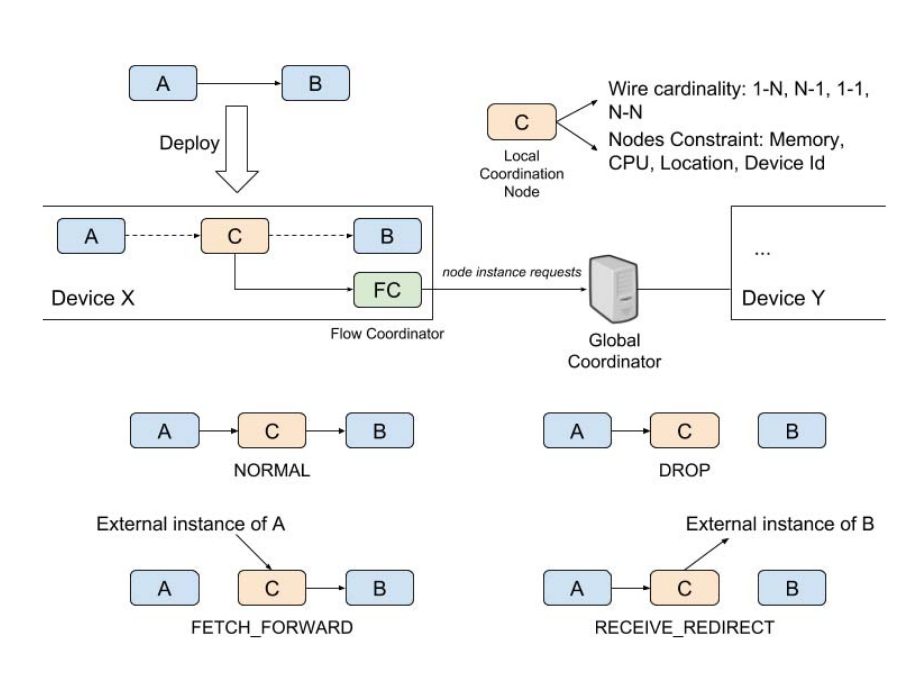
\includegraphics[width=0.8\textwidth]{dnr_exogenous_coordination.png}
\end{figure}

\par Other approach was made in the publication from Szydlo et al. \cite{flow_based_programming_fog}, where they focused on the transformation and decomposition of data flow. Parts of the flow can be translated into the executable parts, such as Lua code. Their contribution includes the concepts of data flow transformation, a new runtime environment called \textit{uFlow} that can be executed on a variety of resource-constrained embedded devices and the integration with the Node-RED platform. 
\par The solution found consisted in the transformation of a given data flow, where the developer chooses the computing operations that will be run on the devices. The operations that will run directly on the devices are implemented in the form of embedded software, using the developed framework \textit{uFlow}, which allows for parts of the flow to be run on heterogenous devices. All this is integrated with NodeRED. The communication between the devices is made only through the cloud, with no support for peer-to-device communication. The results were promising, with the decrease in the number of measurements made by the sensors. However, there is room for improvements, with the automation of the decomposition and partitioning of the initial flow, the detection bottlenecks which will move computations accordingly from the cloud to the fog. Figure \ref{fig:uflow_1} represents a situation of partitioning and assignment of tasks. There are two IoT devices and a Node-RED instance running in the Cloud. The system goal is to measure soil humidity and ambient light. If a button is pressed or fertilizer is needed, an e-mail is sent to the gardener. The partition of computation is made in the assumption that the closer a selected process it to the source of data, the higher the amount of data transmitted between computing operations. After parts of the flow are assigned to specific devices, they are altered in order to be executed by \textit{uFlow} and Node-RED. It is possible to observe in Figure \ref{fig:uflow_1} the results of the transformation process, where the parts of the flow surrounded by a color are executed in the device with the respective color.

\begin{figure}[h]
\caption{Partition and assignment of parts of the flow \cite{flow_based_programming_fog}}
\label{fig:uflow_1}
\centering
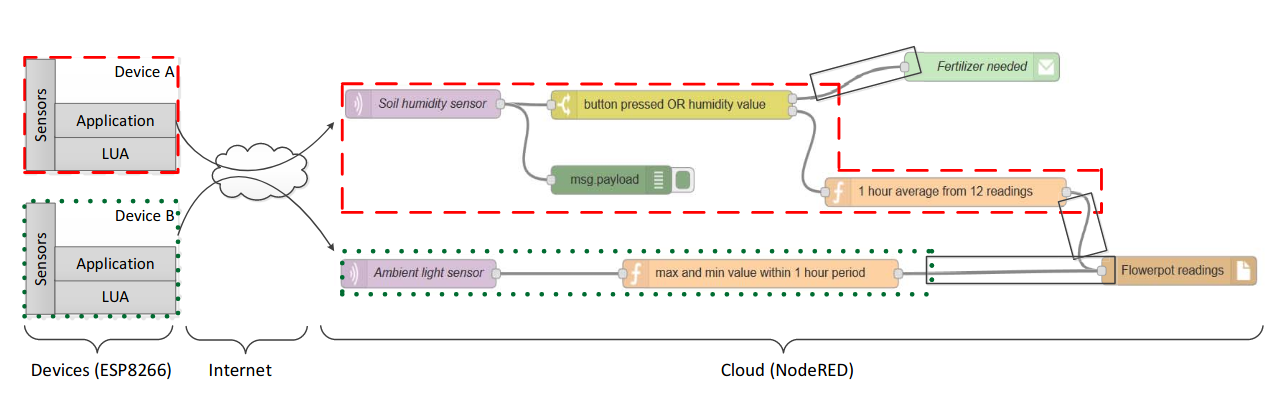
\includegraphics[width=0.9\textwidth]{uflow_1.png}
\end{figure}

\par In 2019, they continued their work with the publication \cite{fog_flow}, where they built the model and engine \textit{FogFlow}, which enables the design of applications able to be decomposed onto heterogeneous IoT environments according to a chosen decomposition schema. To achieve a level of decentralization and heterogeneity, they abstract out the application definition from its architecture and rely on graph representation to provide an unambiguous, well defined model of computations. The application definition should be infrastructure-independent and contain only data processing logic, and its execution should be possible on different set of devices with different capabilities. Several algorithms for flow decomposition were mentioned \cite{algorithm_fog} \cite{ifogsim}, but none were specified in terms of results. Figure \ref{fig:fogflow} represents the \textit{FogFlow} architecture, which is composed by three modules: (1) the \textit{FogFlow} API, which enables the creation of the application definition, (2) the Graph Module, responsible for processing and transforming the application definition into a data flow graph and finally the (3) Execution Model, which translates the graph and generates executables ready to be run on the assigned devices.

\begin{figure}[h]
\caption{\textit{FogFlow} architecture \cite{fog_flow}}
\label{fig:fogflow}
\centering
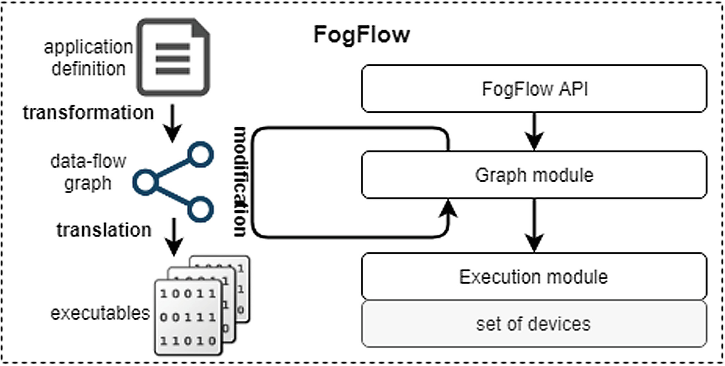
\includegraphics[width=0.8\textwidth]{fogflow.png}
\end{figure}

\par There is another tool with the same name \textit{FogFlow}, but created by Cheng et al. \cite{fogflow_github}. In the first publication related to this tool \cite{fog_flow_easy}, the contributions made were the implementation of a standard-base programming model for Fog Computing and a scalable context management. The first contribution consists in extending the dataflow programming model with hints, ir order to facilitate the development of fog applications. The scalable context management introduces a distributed approach, which allows to overcome the limits in a centralized context, achieving much better performance in terms of throughput, response time and scalability. The \textit{FogFlow} framework focuses in a Smart City Platform use case, separated in three areas: (1) Service Management, normally hosted in the cloud, (2) Data Processing, present in cloud and edge devices and (3) Context Management, which is separated in an device discovery unit hosted in the cloud and IoT brokers scattered in edge and cloud.
\par In more recent work \cite{fog_flow_tool}, \textit{FogFlow} was improved in order to provide infrastructure providers an environment that allows them to build decentralized IoT systems faster, with increased stability and scalability. The architecture can be seen in Figure \ref{fig:fogflow_tool}, where the IoT system is represented by dynamic data flows that are orchestrated between sensors (Producers) and actuators (Consumers). The application is first designed using the \textit{FogFlow} Task Designer, a hybrid text and visual programming environment, which results in an abstraction called Service Template. This abstraction contains specifics about the resources needed for each part of the system. Once the Service Template is submitted, the framework will determine how to instantiate it using the context data available. Each task is associated with an operator, which consists of a Docker image, and its assignment is based on how many resources are available on each edge node, the location of data sources and the prediction of workload. Edge nodes are autonomous since they are able to make their own decisions based on their local context, without relying on the central cloud. \textcolor{red}{Review}

\begin{figure}[h]
\caption{\textit{FogFlow} high level model \cite{fog_flow_tool}}
\label{fig:fogflow_tool}
\centering
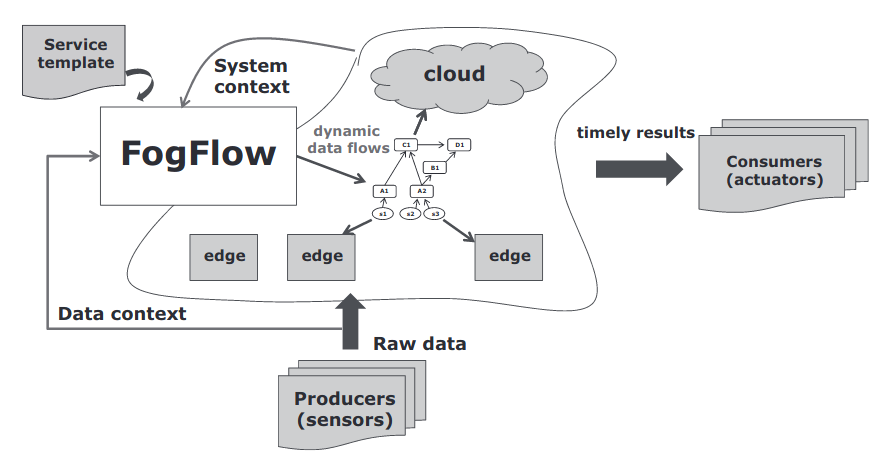
\includegraphics[width=0.8\textwidth]{fogflow_tool.png}
\end{figure}

\par \textcolor{red}{FALAR SOBRE DDFLOW}
\par \textcolor{red}{FALAR SOBRE mobile\_cloud\_heterogeneous e mobile\_cloud?}


%\cite{flow_based_programming_fog}
%\cite{fog_flow}
%\cite{fog_flow_tool}
%\cite{ddflow}


%\cite{mobile_cloud_heterogeneous}
%\cite{mobile_cloud}
%\cite{fog_computing_book}


\section{Summary}

\textcolor{yellow}{\textbf{**TODO**}}


\chapter{Problem Statement} \label{chap:problem_statement}

\section*{}

\minitoc \mtcskip \noindent
This chapter describes the problem, as can be seen in \sectionintroref{sec:current_issues}. In \sectionintroref{sec:desiderata} it is presented the wanted features for the proposed solution and in \sectionintroref{sec:scope} the scope of the project is defined. \sectionintroref{sec:main_hypothesis} contains the hypothesis this dissertation presents. The experimental methodology is outlined in \sectionintroref{sec:exp_meth}. Finally, this chapter is summarized in \sectionintroref{sec:stat_summary} with an overview of the topics mentioned before.

\section{Current Issues}\label{sec:current_issues}

\chapterref{chap:sota} contains several solutions that provide a decentralized architecture in visual programming tools applied to the Internet-of-Things paradigm. However, some of these tools solve specific problems or make assumptions regarding the scale of the system and the constraints of the devices.
We can define the problem in these issues:
\begin{enumerate}
    \item \textbf{Leveraging devices in the network}: since most tools use a centralized architecture, including Node-RED, they do not leverage the devices in the network. Fog Computing introduces a decentralized solution, one that can be applied to Node-RED by distributing the computational tasks across the edge devices.
    \item \textbf{Communication of computational capabilities}: some of the current tools require the developer to manually introduce the resources of each device in the network, which is not a scalable solution. Others have a specific list of services, manually inserted, that the devices can provide. Information about the computational capabilities of the devices in the network is vital for the successful distribution of computation across the devices.
    \item \textbf{Detecting non-availability}: when a device fails or becomes unavailable, it is important for the system to automatically realize and adapt. The majority of current solutions do not possess this feature, which is vital if a system aims to dynamically adapt to changes in the environment.
    \item \textbf{Code generation of sub-flows}: to truly leverage constrained devices, it is important to convert sub-flows or "tasks" into runnable code. Devices that support simple firmware capable of executing code can be used to execute blocks of code, despite their limited capabilities.
    \item \textbf{Provide self-adaption of the system}: devices can fail, as well as the connection between them or even the network. It is important for the system to discover and identify these changes and adapt to them at run-time, in order to keep functioning.
\end{enumerate}

\section{Desiderata}\label{sec:desiderata}
Desiderata is a Latin word that translates to "\emph{things wanted}". In the context of this document, this section contains requirements wanted in a solution that aims to solve all the issues identified in \sectionref{sec:current_issues}. The requirements are the following:

\begin{description}
    \item [D1: Communicate computational capabilities of devices connected] so that this information can be sent to an orchestrator that will decompose the total computation workload based on this data.
    \item [D2: Decomposition and partition of computation] so that the total computational requested can be distributed through all the devices in the network, using information about the computational capabilities and availability of the devices in the network.
    \item [D3: Convert computational tasks into runnable code] so that each computational task can be executed in edge and fog devices, which contain limited resources.
    \item [D4: Provide self-adaptation of the system] so that it can adapt to the non-availability of resources or even appearances of new devices.
\end{description}

\section{Scope}\label{sec:scope}

The focus of this dissertation is the development of a prototype that allows for a decentralized orchestration of an IoT system. Despite security being a critical feature, it is considered a secondary goal, allowing the dissertation to focus on its primary goals. The scope of the project is a home automation system, where its devices have firmware capable of running  MicroPython code and accepting custom code. They also need to be able to communicate their capabilities to an orchestrator.

%\section{Use Cases}\label{sec:use_cases}

\section{Main Hypothesis}\label{sec:main_hypothesis}

This dissertation is built around the following hypothesis:

\begin{quote}
    \emph{``Given an IoT system with several heterogeneous devices connected, capable of running custom code, a decentralized architecture is more resilient, efficient and scalable than a centralized one.''}
\end{quote}

The attributes presented in the hypothesis will be measure against a system using the current development branch of Node-RED. These attributes consist of:

\begin{itemize}
    \item \textbf{Resilience} means the system's capability to adapt to failures and changes. It will be measured by injecting failures and measuring the recovery patterns.
    \item \textbf{Efficiency} how fast the system can execute the logic of the system and communicate between nodes. The efficiency of a system is measured by the latency when reacting to system events. 
    \item \textbf{Elasticity} specifies how a system can grow and shrink. This attribute will be tested by increasingly adding or removing devices in different scenarios and assessing the overall system's behavior.
\end{itemize}

\section{Experimental Methodology}\label{sec:exp_meth}

In the interest of validating whether or not the solution implemented achieves the \emph{desiderata} and solves the current issues, we will develop test scenarios and experiments that use both virtual and physical devices. Each one of the test scenarios will measure the one or more requirements proposed in Section \ref{sec:desiderata}. Lastly, the attributes mentioned in Section \ref{sec:main_hypothesis} will be evaluated with the implement solution, in order to validate the given hypothesis.

\section{Summary}\label{sec:stat_summary}

\sectionref{sec:current_issues} starts by presenting issues and lack of features not fully present in the current tools presented in the State of the Art \chapterref{chap:sota}. \sectionref{sec:desiderata} presents a \textit{desiderata} that aims to fix the issues presented in \sectionref{sec:current_issues}. The hypothesis of this dissertation is presented in \sectionref{sec:main_hypothesis}, as well as an experimental methodology to prove it, in \sectionref{sec:exp_meth}.

%\chapter{Solution} \label{chap:solution} \minitoc

\section*{}

This chapter describes how the problem presented in Chapter \ref{chap:problem_statement} was solved by stating the solution implemented and the reasons for the choices taken.  \textbf{\textcolor{red}{End with the sections' descriptions}}

\section{Overview}\label{sec:solution_overview}

The goal of this dissertation is to modify Node-RED in order to decentralize its architecture, taking advantage of the capabilities of external devices, no matter how limited they are.

The solution implemented was to use the Node-RED instance to orchestrate the decentralization and send tasks to other devices in the network. The devices make themselves known by announcing their address and capabilities to a registry node running in Node-RED. Consequently, Node-RED assigns nodes to devices and communicates each node's assignment via WiFi. Due to the devices' limitations, they cannot run an instance of Node-RED, so Node-RED needs to convert nodes in Javascript to other language that can be interpreted by these devices. The implemented solution requires a Micropython port and a HTTP server that receives and executes a micropython script created by the Node-RED. This script contains the tasks assigned to a device, translated into micropython. 

After the first deployment of the system, the Node-RED instance manages the state of each device, allowing the system to re-orchestrate if any of the devices becomes unavailable.

\begin{figure}[h]
\centering
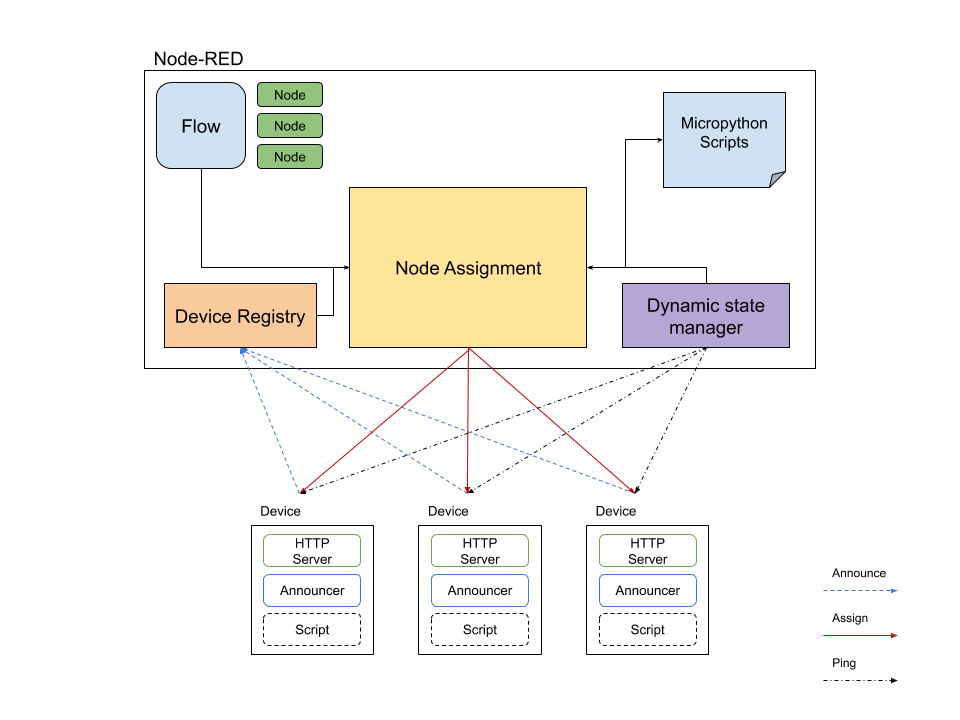
\includegraphics[width=\textwidth]{overview.png}
\caption[Solution's overview]{An overview of the solution}\label{fig:solution_overview}
\end{figure}

\textcolor{blue}{Explain and improve graphic}


\section{Implementation details}\label{sec:implementation_details}

\subsection{Device registry}\label{sec:registry}

When a device becomes available it sends information about itself to a MQTT topic. This information contains the device's IP address, their capabilities and their status - if the device has failed before. In its turn, Node-RED contains a Node called \textit{Registry} that listens to the announcements MQTT topics and saves the devices information. If this node is connected to a orchestrator node, each new device is communicated so that the orchestration can be updated.

When a device has an Out of Memory error, it triggers a fail-safe, where it reboots the HTTP server, stop running any script and restarts all communications. After this action, the device announces itself again but with a flag that indicates that it has failed. This way, Node-RED knows that a device is active but not running any code, and that it possible failed due to too much work. In that case, Node-RED will assign less nodes to the device, reducing the chances of causing another Out of Memory error.

\textcolor{blue}{What is there more to add? Maybe this section is not here, add to other place}

\subsection{Devices setup for decentralization support}\label{sec:devices_decentralization}

The first problem approached in this thesis was finding a way to take advantage of devices with few computational resources, integrating them in a IoT system. The goal was to make these devices execute scripts of code and communicate with other devices, despite their capability limitations. In order to limit the number of type of different devices capable for this aim, only ESP8266 and ESP32 chips were used, since they have connectivity capabilities such as an WiFi chip. In terms of testing, the environment in the devices was replicated in Docker container running the Unix port of micropython.

\subsubsection{Solution overview}

As it was mentioned before in Section \ref{sec:solution_overview}, the devices in the system run a micropython port that allows the execution of scripts written in micropython. This solution is lightweight and extensible. Since these devices need to receive different types of tasks throughout their execution, their firmware includes an HTTP server responsible for receiving scripts of code, saving and executing them. Besides this functionality, it was also implemented an endpoint that returns the state of the device, as well as the announcing mechanism, explained in Section \ref{sec:registry}.

Several micropython libraries were used, more specifically uasyncio and micropython-mqtt. The uasyncio library allowed the implementation of asynchronous operations, critical for the execution of the given script as well as maintaining the HTTP server running and non-blocking.

The firmware also includes a fail-safe mechanism, safeguarding against \textit{out-of-memory} errors that may happen during the lifespan of the device. This mechanism resets all running tasks and recovers the HTTP server and communication channels. This an important feature due to the high probability of these error's occurrence, since the devices have limited memory. 

However, the solution is not perfect and has several limitations, such as:

\begin{itemize}
    \item Support only for mqtt QOS 0 and 1, due to limitations in the MQTT library used. 
    \item ESP8266 memory limitations, where the fail-safe is not possible if the given a script too big.
\end{itemize}

\textcolor{blue}{Maybe add an image explaining the firmware, idk}

\subsection{Node-RED decentralization of computation}\label{sec:node_red_decentralization}

Node-RED is a centralized tool by design, which takes advantage of events to allow communication between nodes in a flow. To implement a decentralized architecture, some changes were made to the Node-RED runtime. These changes consisted in implementing a new way of communication between nodes, detailed in Section \ref{sec:mqtt_support}, as well as implementing specific nodes responsible for the orchestration and registry of devices. \textcolor{blue}{complete later}

\subsubsection{MQTT node communication support}\label{sec:mqtt_support}

Node-RED nodes communicate using events, where a node only communicates with nodes it is wired to. The communication is one way, with the node only sending data to the nodes it is connected to by output. These output wires are used to access the nodes the message must be sent to, and their \texttt{receive()} method is called. This method triggers the event \texttt{emit} which will the caught by a specific method of each node, implementing its own logic.

\textcolor{blue}{Insert code block with example? Or an image explaining?}

This implementation is local and Javascript specific, making it impossible to be used in a decentralized architecture where nodes will be executed outside the Node-RED instance. It was necessary to implement a way of communicating between nodes external to Node-RED that could be supported by low capacity devices. The solution found was MQTT, which fits as a good solution by its low cost and high popularity.

Node entities were changed to support MQTT instead of events, subscribing to topics created at run-time that match the wires between the nodes. Support for sub-flows was also implemented.

\textcolor{blue}{Insert here image that shows a flow with wires and the respective flow with examples of topics}

\subsubsection{Code generation}\label{sec:code_generation}

\textcolor{blue}{Talk about each node code generation, the support for multiple node scripts in one script. Talk about limitation that different nodes on one script, even consecutive nodes, require to communicate with each other by MQTT topics}

As explained above, due to the limitations of the devices used, it was necessary to translate Node-RED nodes, written in Javascript, to micropython code. Along with that, it was also necessary to support multiple nodes in one script, making it necessary to create a generalized script that could fit any type of node.

The implemented solution consists of each node having specific methods related to their functionality and one point of input and output. Since the communication is made by MQTT, as specified in Section \ref{sec:mqtt_support}, the only input a Node can have is in its topics. The same for the output logic. A exception to this is in nodes that are sources, meaning that they generate input and don't receive it. 

The creation the script is made after the assignment of nodes to devices, and each device has its respective script created. The process consists of creating the script with the code of all the assigned nodes and a general code that ties up the script. This general code is responsible for subscribing to all the input topics of all the nodes, stopping the script's processes and forwarding the MQTT messages to the respective node's code.

\textcolor{blue}{Insert Node-RED flow example and the respective micropython script}

\textcolor{red}{Talk about the limitation of communication of two nodes with direct communication being assigned to the same device and still having to communicate to each other via MQTT instead of just calling each other through code.}

\subsubsection{Custom nodes}\label{sec:custom_nodes}

As mentioned before, the orchestration and registry logic are contained in two custom nodes. Besides this two nodes, several others were created in order to test the system and simplify the code generation and others that already existed were altered. 

The nodes created are: (a) If Node, that receives an input and verifies if it complies with all the given rules, returning true or false, (b) And Node, that receives a given number of inputs and verifies if all of them are true or false, returning the corresponding boolean, (c) Temperature-Humidity Node, that read the temperature and humidity from a DHT sensor present in a specific pin, (d) Failure Node, that raises a MemoryError exception, (e) Nothing Node, that simply redirects the received message in its input to its output, and (f) MQTT In and Out Nodes, that subscribe and publish MQTT topics, respectively.

\subsubsection{Computation Decentralization}\label{sec:node_red_computation_decentralization}

The focal point of this dissertation is the decentralization of computation. Given a set of tasks, it must assign them to available devices, ensuring that they will be performed.

To implement this assignment, each device has a set of capabilities, which communicate what the device is capable of doing or accessing, \textit{e.g.} executing micropython code, assessing a DHT sensor, etc. This capabilities are communicated to the orchestrator by the registry, which receives this information by the devices themselves, as is explained in the Section \ref{sec:registry}. 

Besides this, each node has two properties: Predicates and Priorities. Similar to the Kubernetes logic of assigning containers to machines, the predicates dictate constraints that cannot be violated, and priorities are requests that are advisable and recommended but can be violated if impossible to comply. 

The assigning algorithm uses the devices capabilities and each node's predicates and priorities to assign nodes to devices. With a a greedy approach, ir filters the devices that comply with each node's predicates and assigns the one with a higher value of a heuristic. This heuristic takes into account the number of priorities the device can provide, as well as the number of already assigned nodes the device has. The goal is to assign each node to the best possible device, spreading the tasks through all the available devices.

\textcolor{blue}{Insert here assigning algorithm pseudocode}
% node
% bestIndex = 0

% for device in devices:
%     if not all node predicates in device tags: return
%     intersectionIndex = (nº of node priorities in device tags)/(nº node priorities)
    
%     matchIndex = 
%         intersectionIndex * 0.5 + 
%         (1/( nodes assigned to the device) + 1) * 0.4 +
%         (nº of node priorities in device tags/ device tags) * 0.1
    
%     if matchIndex > bestIndex:
%         bestIndex = matchIndex
%         device is the best choice for node

After assigning all nodes to a specific device, a micropython script is generated to each device, as explained in Section \ref{sec:code_generation}. Due to the limitations in memory of the devices, the quantity of nodes assigned to a device may be excessive to its capabilities. In that case, the device will fail-safe and return an error to the assignment request. The orchestrator will receive this information and repeat the process, assigning less nodes to the devices that returned a memory error. If a device does not return any response, the orchestrator will assume that the device is unavailable and not assign any node to it.

\textcolor{blue}{Add an example of an assignment (JSON file) or/and a visual alternative with blocks and labels. With devices with capabilities and the assigned nodes predicates and priorities.}

The process explained above is triggered by four types of events: (1) start of the system, when there is already a defined flow in the configuration, the assignment start after a period of 3 seconds, to give time for the devices to be registered by the registry node; (2) deployment of the entire flow using the Node-RED editor or API; (3) appearance of a new device, with the announcement of it to the registry node; (4) failure or recovery of a device, communicated by the dynamic state management mechanism, detailed in Section \ref{sec:dynamic_state_management}.

\textcolor{blue}{Maybe add an image of the process, with the possible steps that can trigger an announcement, or the flow of the process}

However, due to the use of a greedy algorithm, there are some limitations in the assignment. Besides not resulting in the best possible solution, there is specific situations that can result in the impossibility of complying with the constraints imposed by nodes. For example, given a scenario where the number of devices is small for the quantity of nodes, resulting in the devices being at the limit of their memory capabilities. If there is a node which constraints can only be complied by one device, but that one device already has the maximum number of nodes it can handle, the assignment is not possible.

\textcolor{red}{Falar tmb (?) que o algoritmo não tem em conta o facto de dois nós seguidos ficarem no mesmo dispositivo - isto agora não tem mt impacto pq toda a comunicação é feita por MQTT mas uma possibilidade era 2 nós seguidos ficarem no mesmo dispositivo e comunicarem chamando a função do outro em vez de ser por MQTT}

\subsubsection{Dynamic state management}\label{sec:dynamic_state_management}

After the assignment process, each device is doing their part to allow the system to work as expected. However, given the simplicity of the devices used, such as ESP8266s and ESP32s, they are prone to failures, with possible causes ranging form power loss to faulty hardware, among others.

Due to this limitations, the orchestrator periodically pings the devices in the system, registering any change in their state. If a state is noticed, the orchestrator will repeat the process of assignment taking into account the changes in the device's availability. This detects not only non-availability but also if a device becomes active again after a failure.

\textcolor{blue}{Don't know what to add more}

\subsubsection{Limitations}\label{sec:limitations}

\begin{itemize}
    \item Number of nodes that support micropython code generation is small
    \item Duplicate messages when redeploying the totality of the flow (maybe fixable later)
    \item Re-orchestration only supported when deploying the entire instance (all flows)
    \item Nodes do not stop working when the Node-RED instance is stopped
    \item Script generated does not take into account nodes that communicate directly, forcing all communications through MQTT instead of a node calling the method of another with the output as argument.
    \item Assignment algorithm does not take into account the assignment of sequential nodes in the same device.
\end{itemize}
 
%\chapter{Evaluation} \label{chap:evaluation} \minitoc

\section*{}

This section evaluates how the solution developed proves the hypothesis proposed in Chapter \ref{chap:problem_statement}.

\textcolor{blue}{Complete...}

% First, an explanation of the scenarios will be made, as well as their relation to the features developed and their advantages. 

\section{Scenarios and Experiments}\label{sec:scenarios_experiments}

The testing of the proposed solution diverged in two different scenarios. The first simulates physical devices with the use of Docker containers running the Unix port of micropython, allowing the construction of scalable scenarios with minimal costs. The second scenario uses physical devices, such as ESP8266 and ESP32, connected to the same Wi-Fi.

\begin{enumerate}
    \item A room has 3 sensors that give temperature and humidity readings every minute. There’s a virtual sensor that compares the results (of both temperature and humidity) and triggers depending on some configured thresholds. An AC uses those readings to decide (a) if it switches on/off, (b) its operating mode: cool, heat, and dehumidify. The Minimal Working System (MWS) consists in (a) one temperature sensor, (b) one humidity sensor, (c) one node capable of making the decision, and (d) working communication channels amongst them.
    \item 20 devices, where each device redirects its input to its output. \textcolor{red}{improve}
\end{enumerate}

The first scenario aims to test the features of the developed solution with a moderately simple Node-RED flow, taking advantage of the nodes developed for micropython code generation support. The second scenario allows the comparison of the developed solution to the already existing solutions.

\textcolor{red}{Refactor this enumeration, with some explaining of some terms}

\textbf{Scenario 1}:
\begin{enumerate}
    \item \textbf{Sanity check.} All tasks are simple readings and forwarding, no compensation or other fault-tolerance strategy. Each sensor does its own thing. Orchestration is centralized. We expect all roundtrips to take less than the smallest part that can be resolved (measurement capability, which we estimate to be <1s).
    \item \textbf{Re-orchestration.}
        \begin{itemize}
            \item \textbf{Experiment A.} MWS is achieved via multiple possible configurations by selective (provoked) device failure (fail-stop);
            \item \textbf{Experiment B.} Inconsistent device behaviour, e.g. appear and disappear in shorter intervals lower that the time needed for orchestrating convergence (OCT), that leads to activity impacting the MWS;
            \item \textbf{Experiment C.} With 20 devices, each one with different processing capabilities. During orchestration, some devices will develop an out-of-memory error because they can't process all the processing tasks assigned to them, specifically the size of the script given. The orchestrator decides to send less tasks to these devices. The system will converge in a working solution. \textit{This scenario will be implemented with a modified device script. When devices receive a script, it will generate a memory error if the length of the script passes a certain threshold. This simulates the memory constraints of devices when receiving a file to big.}
            \item \textbf{Experiment D.} With 20 devices, some of them have a memory leak with an unknown cause. After random time Random(t0,t1), these problematic devices stop working with an out-of-memory error. The orchestrator thinks that the devices can't handle the quantity of processing tasks assigned to them, so in the re-orchestration it will assign fewer tasks. Since these devices will always break, the orchestrator will eventually not consider these devices in the assignment of nodes. \textit{This scenario will be implemented with a modified device script that will trigger an out-of-memory error after a random period after executing the given tasks.}
            \item \textbf{Experiment E.} With 20 devices, there is a device that is sensitive to a particular node, which causes the device to give out an out-of-memory error. The orchestrator will potentially assign this node to the specific device. When the device gives out the out-of-memory error, the orchestrator will eventually converge in a solution where the node is not assigned to the particular device, and the system will converge.  \textit{These out-of-memory errors will be simulated with the use of a failure node that forces an \texttt{MemoryException} in the device.}
        \end{itemize}
        Verifies that:
        \begin{enumerate}
            \item \textbf{Restrictions (predicates) are enforced.} Check that possible configurations lead to solutions that enforce defined predicates;
                \begin{enumerate}
                    \item Temperature and humidity might coexist in the same, or in dedicated, devices;
                \end{enumerate}
            \item \textbf{Priorities are honored.} Check that all specified priorities were taken into account, and only violated if necessary;
                \begin{enumerate}
                    \item Priority is given to edge devices, but fog and cloud can be used;
                    \item Priority is given to the maximum level of decentralization, but some centralization can be used.
                \end{enumerate}
        \end{enumerate}
    \item \textbf{Latency.} Make devices selectively slow and check the consequences; might impact OCT and MWS. ? \textcolor{red}{was not implemented}
\end{enumerate}

\textbf{Scenario 2}:
With the use of 20 physical devices, both ESP8266 and ESP32, implement a line topology, where a message is sent to a starting device, that will propagate it to its output. All the devices implement this propagation logic, which results in the initial message reaching the end of the line. The propagation time is measured, starting when the message is sent and ending when the message reaches the last node.
This experience is implemented in several environments:
\begin{enumerate}
    \item \textbf{Node-RED original}. Runs the experiment in the original Node-RED, using the default option (events) as the communication channel between nodes.
    \item \textbf{Node-RED + MQTT}. Run the experiment in Node-RED, using MQTT as the communication channel between nodes.
    \item \textbf{Node-RED modified + Dockers (same host)} Runs the experiment in the modified version of Node-RED, with each node assigned to a different virtual device, running in a Docker container. The virtual devices are in the same host machine running the MQTT server instance.
    \item \textbf{Node-RED modified + Dockers (different host)} Runs the experiment in the modified version of Node-RED, with each node assigned to a different virtual device, running in a Docker container. The MQTT server instance is in a different host machine from the one running the virtual devices. All machines are connected through Wi-Fi.
    \item \textbf{Physical + MQTT} Runs the experiment in physical devices without the developed firmware. Each device runs a simple micropython script that executes the wanted behaviour, communicating by MQTT. No Node-RED is used.
    \item \textbf{Node-RED modified + MQTT + Physical + Firmware} Runs the experiment with the developed solution, with each node assigned to a different physical device running the developed micropython firmware. All communicating is made using MQTT.
\end{enumerate}

\section{Discussion}\label{sec:evaluation_discussion}

\textcolor{blue}{For each experiment, analyse the data and discuss the results - many graphs, more tables and lots of text - fun times and very little time!}

\subsection{Scenario 1}\label{sec:discussion_scenario1}

\textcolor{blue}{Talk about the results of the scenario1 experiments, with graphs, prints of the scenario in Node-RED and conclusions}

\subsection{Scenario 2}\label{sec:discussion_scenario2}

As mentioned previously, several experiences were made to compare the developed solution to existing ones. To this end goal, a simple experiment of passing a message through several devices was implemented and the time the message takes to pass through all the devices was measured. The implementation of the scenario in the Node-RED tool is shown in Figure \ref{fig:scenario2_node_red}. The \textit{nothing} nodes execution consists of only redirecting their input to their output. The message consisting of the current timestamp is inserted into the system by the \textit{inject} node with user input, and the same message is showcased by the \textit{debug} node, the green one.

\begin{figure}[h]
\centering
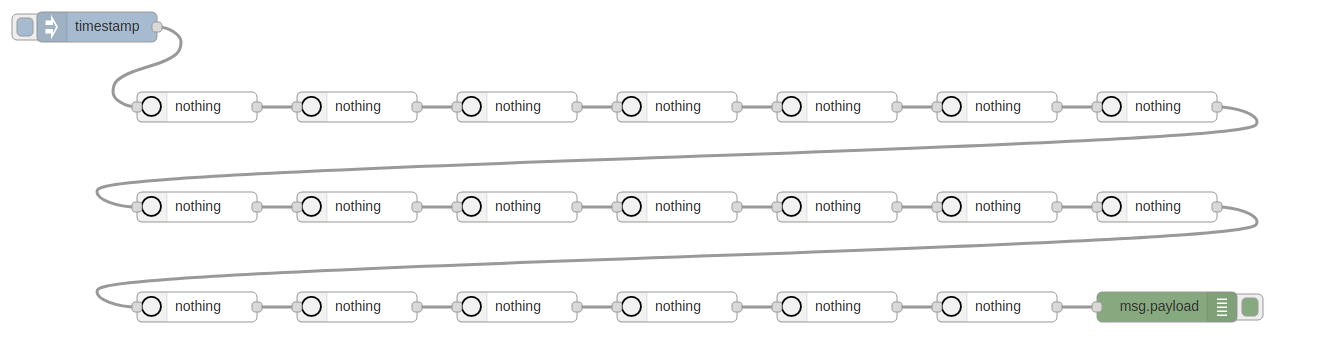
\includegraphics[width=\textwidth]{scenario2.png}
\caption[Solution's overview]{Node-RED implementation of scenario 2}\label{fig:scenario2_node_red}
\end{figure}

This same setup was replicated in several environments, as mentioned before. Each experiment was replicated 10 times, resulting in the data seen in Table \ref{tab:scenario2_table} and visually detailed in Figure \ref{fig:scenario2_candlestick}.

\captionsetup{belowskip=12pt,aboveskip=4pt}
\begin{table}[ht]
    \centering
    \resizebox{0.8\textwidth}{!}{%
    \begin{tabular}{ l  c  c  c  c }
        \toprule
        \textbf{Label} & \textbf{Min} & \textbf{Q2} & \textbf{Q3} & \textbf{Max}\\
        \midrule
        Node-RED original & 3 & 10 & 13.25 & 15 \\
        Node-RED + MQTT & 134 & 430.5 & 711.25 & 883 \\
        Node-RED modified + Dockers (same host) & 1217 & 1318 & 1573.75 & 1665 \\
        Node-RED modified + Dockers (different host) & 1445 & 2536 & 2708 & 3059 \\
        Physical + MQTT & 3616 & 4142 & 4372 & 4452 \\
        Node-RED modified + MQTT + Physical + Firmware & 4168 & 4569 & 5087.75 & 5940 \\
        \bottomrule
    \end{tabular}
    }
    \caption{Scenario 2 results}
    \label{tab:scenario2_table}
\end{table}{}

\begin{figure}[h]
\centering
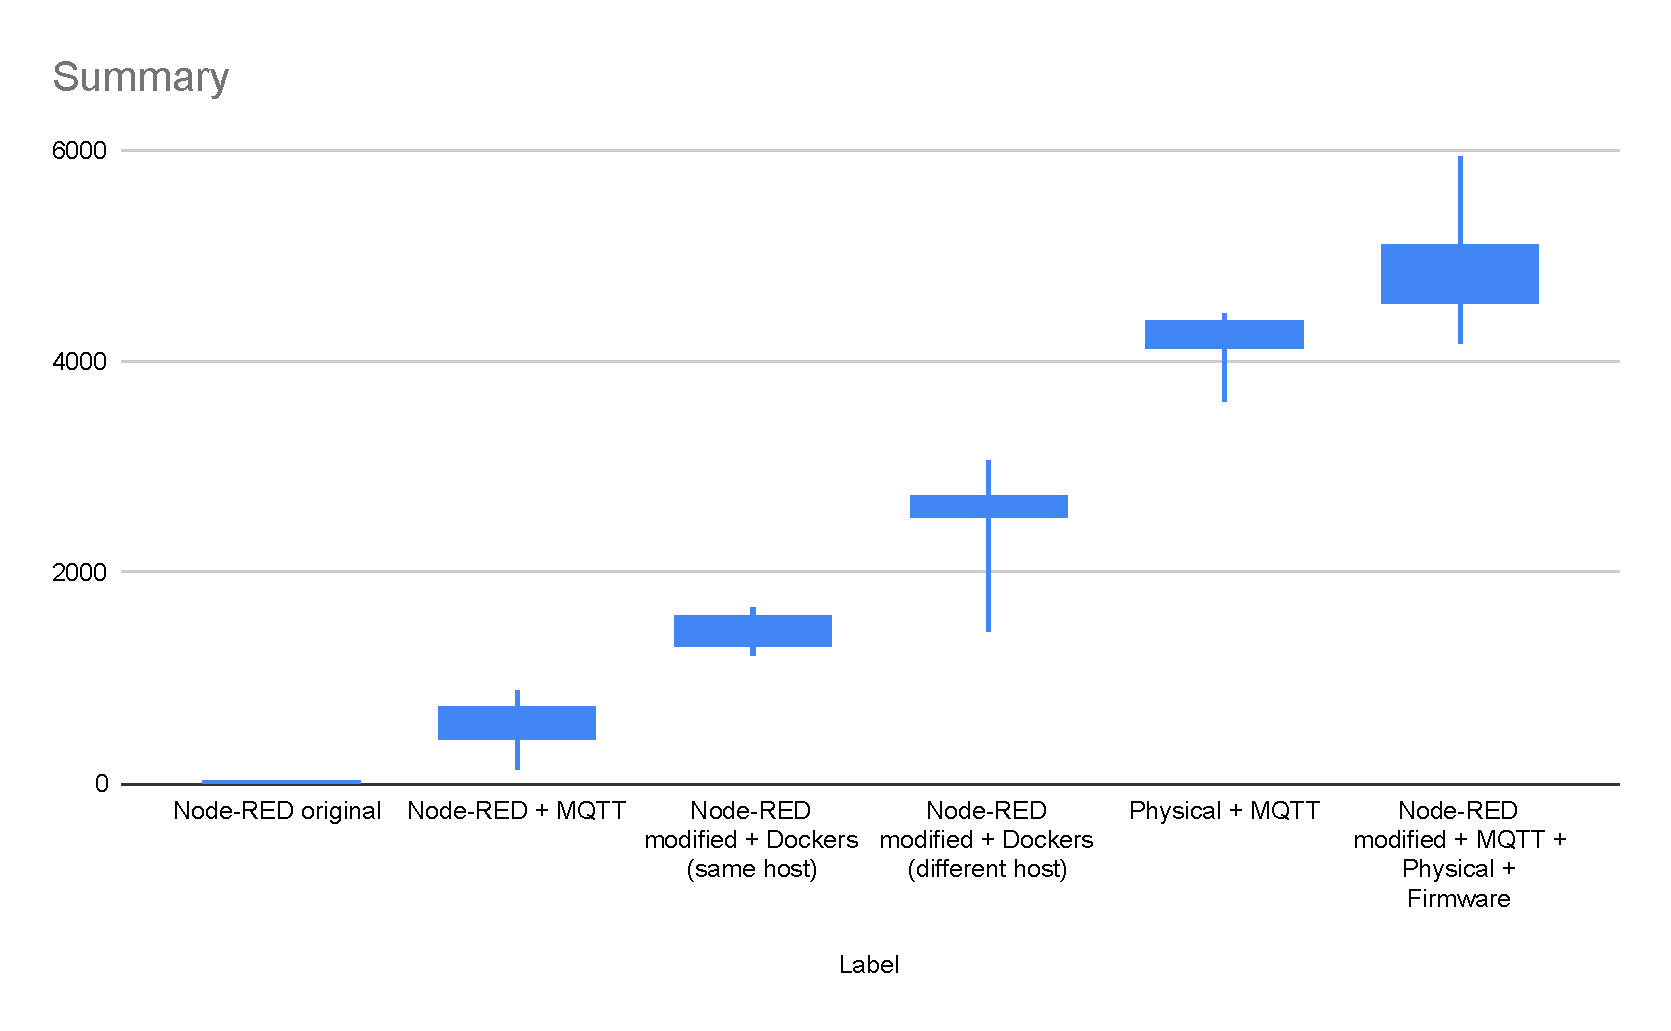
\includegraphics[width=\textwidth]{scenario2_graph.pdf}
\caption[Scenario 2 results]{Scenario 2 results}\label{fig:scenario2_candlestick}
\end{figure}

With the given results, we can conclude several things. 

\textcolor{blue}{Talk about how the communication stack hinders the speed of the solution - aka, different host, as well as the micropython firmware also hinders}

\textcolor{red}{Add other tables with the timestamps in the annex}

\subsection{Overview}\label{sec:discussion_overview}

\textcolor{blue}{Overview of the evaluation of the system, with conclusions of the evaluation of the system as a whole}

\section{Conclusions}\label{sec:evaluation_conclusions}


\chapter{Conclusions} \label{chap:concl}

\section*{}


As the number of devices connected to the internet increases, it is important to leverage their capabilities and modify the way systems are built to take advantage of these resources. It is also important to allow end-users with no programming experience to build Internet-of-Things (IoT) systems, with the use of visual programming tools. These tools make the building process easier, reducing the knowledge of programming concepts needed.

Despite the existence of a considering number of visual programming tools applied to IoT, the majority of these tools are centralized. This centralization hinders the resiliency of the system, as the unit responsible for the execution of most or all of the computation is a single point of failure. If this unit or the network fails, the system stops being functional. Another issue of this type of architecture is the lack of usage of the computational capabilities of the rest of the devices in the system.

During the analysis of the state of the art, some issues and missing features were identified, which this dissertation aims to correct. The tools found that possess a decentralized architecture have limiting characteristics such as assumptions about what is a constrained device regarding computational capabilities, lack of open source licenses and simplification of the approach taken to the decomposition and assignment of tasks.

This dissertation aims to solve these issues by expanding an already popular visual programming tool, Node-RED, with a decentralized approach that focuses on leveraging all the devices, even ones that only support the execution of simple blocks of code. The expected result is a decentralized system that can self-adapt to run-time conditions and decomposes the given computations into independent tasks, which are assigned to devices. The assignment's goal is to increase the efficiency of the system, reducing latency and distributing CPU usage.  


\section{Difficulties}
\begin{itemize}
    \item Problemas de memória e espaço dos ESPs para execução de scripts de micropython com 3+ nós (ESPs lançam erros de alocamento de memória se o script enviado é maior que um certo nº de bytes ou ao fazer redeploy de scripts de médio tamanho). - Alternativas: failsafe (implementado e funcional), pyc (não existe para micropython mas existe o .mpy. No entanto, precisa de ser executado para gerar um .mpy a partir de um .pt, o que não se aplica à solução atual), ota (não existem boas soluções para micropython)
    \item Necessidade de implementar novos nós para situações de teste
    \item Node-red não suporta comunicação de mqtt entre nós de raíz. Node-red teve de ser adaptado para que a comunicação entre nós fosse feita desta maneira.
    \item Modificar scritps e suporte para o port para Unix do micropython - muitas diferenças, limitações e criação de muitos bugs.
    \item Limitações das bibliotecas usadas de micropython, especificamente nas bibliotecas de mqtt e operações assíncronas.
\end{itemize}{}

%\section{Contributions}

%\section{Conclusions}

%\section{Future Work} 

%% comment next 2 commands if numbered appendices are not used
%\appendix
%\chapter{Scenario 2 Results} \label{ap:scenario2_tables}

\captionsetup{belowskip=12pt,aboveskip=4pt}
\begin{table}[h]
    \centering
    \begin{tabular*}{\textwidth}{ l @{\extracolsep{\fill}} l  l }
        \toprule
        \textbf{Start} & \textbf{End} & \textbf{Delta}\\
        \midrule
        1591876328759 & 1591876328770 & 11 \\
        1591876329440 & 1591876329448 & 8 \\
        1591876329991 & 1591876329994 & 3 \\
        1591876330539 & 1591876330554 & 15 \\
        1591876331106 & 1591876331120 & 14 \\
        1591876331658 & 1591876331667 & 9 \\
        1591876332192 & 1591876332200 & 8 \\
        1591876332710 & 1591876332721 & 11 \\
        1591876333222 & 1591876333237 & 15 \\
        1591876333779 & 1591876333787 & 8 \\
        \bottomrule
    \end{tabular*}
    \caption{Node-RED original results}
    \label{tab:node_red_original}
\end{table}{}

\captionsetup{belowskip=12pt,aboveskip=4pt}
\begin{table}[ht]
    \centering
    \begin{tabular*}{\textwidth}{ l @{\extracolsep{\fill}} l  l }
        \toprule
        \textbf{Start} & \textbf{End} & \textbf{Delta}\\
        \midrule
        1591877265187 & 1591877265346 & 159 \\
        1591877266172 & 1591877267055 & 883 \\
        1591877267564 & 1591877267698 & 134 \\
        1591877268318 & 1591877268955 & 637 \\
        1591877269424 & 1591877269783 & 359 \\
        1591877270361 & 1591877271117 & 756 \\
        1591877271635 & 1591877272012 & 377 \\
        1591877272630 & 1591877273132 & 502 \\
        1591877273645 & 1591877273996 & 351 \\
        1591877274541 & 1591877275277 & 736 \\
        \bottomrule
    \end{tabular*}
    \caption{Node-RED + MQTT results}
    \label{tab:node_red_mqtt}
\end{table}{}

\captionsetup{belowskip=12pt,aboveskip=4pt}
\begin{table}[ht]
    \centering
    \begin{tabular*}{\textwidth}{ l @{\extracolsep{\fill}} l  l }
        \toprule
        \textbf{Start} & \textbf{End} & \textbf{Delta}\\
        \midrule
        1591877987030 & 1591877988695 & 1665 \\
        1591877989911 & 1591877991177 & 1266 \\
        1591877992272 & 1591877993595 & 1323 \\
        1591877994286 & 1591877995817 & 1531 \\
        1591877996305 & 1591877997618 & 1313 \\
        1591877998049 & 1591877999307 & 1258 \\
        1591877999734 & 1591878001322 & 1588 \\
        1591878001638 & 1591878002855 & 1217 \\
        1591878003397 & 1591878004643 & 1246 \\
        1591878005113 & 1591878006703 & 1590 \\
        \bottomrule
    \end{tabular*}
    \caption{Node-RED modified + Dockers (same host) results}
    \label{tab:node_red_docker_same}
\end{table}{}

\captionsetup{belowskip=12pt,aboveskip=4pt}
\begin{table}[ht]
    \centering
    \begin{tabular*}{\textwidth}{ l @{\extracolsep{\fill}} l  l }
        \toprule
        \textbf{Start} & \textbf{End} & \textbf{Delta}\\
        \midrule
        1591908868087 & 1591908870410 & 2323 \\
        1591908871443 & 1591908873803 & 2360 \\
        1591908874380 & 1591908877085 & 2705 \\
        1591908877629 & 1591908880338 & 2709 \\
        1591908880878 & 1591908883937 & 3059 \\
        1591908884472 & 1591908887147 & 2675 \\
        1591908887651 & 1591908889096 & 1445 \\
        1591908889803 & 1591908892200 & 2397 \\
        1591908892693 & 1591908894158 & 1465 \\
        1591908894846 & 1591908897623 & 2777 \\
        \bottomrule
    \end{tabular*}
    \caption{Node-RED modified + Dockers (different host) results}
    \label{tab:node_red_docker_different}
\end{table}{}

\captionsetup{belowskip=12pt,aboveskip=4pt}
\begin{table}[ht]
    \centering
    \begin{tabular*}{\textwidth}{ l @{\extracolsep{\fill}} l  l }
        \toprule
        \textbf{Start} & \textbf{End} & \textbf{Delta}\\
        \midrule
        1591904836329 & 1591904840130 & 3801 \\
        1591904844918 & 1591904849155 & 4237 \\
        1591904850127 & 1591904854579 & 4452 \\
        1591904855324 & 1591904859754 & 4430 \\
        1591904860483 & 1591904864559 & 4076 \\
        1591904865164 & 1591904869180 & 4016 \\
        1591904869770 & 1591904873905 & 4135 \\
        1591904874557 & 1591904878706 & 4149 \\
        1591904879318 & 1591904882934 & 3616 \\
        1591904888813 & 1591904893230 & 4417 \\
        \bottomrule
    \end{tabular*}
    \caption{Physical + MQTT results}
    \label{tab:physical_mqtt}
\end{table}{}

\captionsetup{belowskip=12pt,aboveskip=4pt}
\begin{table}[h]
    \centering
    \begin{tabular*}{\textwidth}{ l @{\extracolsep{\fill}} l  l }
        \toprule
        \textbf{Start} & \textbf{End} & \textbf{Delta}\\
        \midrule
        1591878582050 & 1591878587990 & 5940 \\
        1591878589026 & 1591878593492 & 4466 \\
        1591878594105 & 1591878598640 & 4535 \\
        1591878599238 & 1591878603841 & 4603 \\
        1591878604570 & 1591878608765 & 4195 \\
        1591878609340 & 1591878614220 & 4880 \\
        1591878615030 & 1591878620187 & 5157 \\
        1591878620870 & 1591878625038 & 4168 \\
        1591878625718 & 1591878630967 & 5249 \\
        1591878631560 & 1591878635880 & 4320 \\
        \bottomrule
    \end{tabular*}
    \caption{Node-RED modified + MQTT + Physical + Firmware}
    \label{tab:nr_mqtt_physical_firmware}
\end{table}{}

%%----------------------------------------
%% Final materials
%%----------------------------------------

%% Bibliography
%% Comment the next command if BibTeX file not used
%% bibliography is in ``myrefs.bib''
\PrintBib{myrefs}

%% Index
%% Uncomment next command if index is required
%% don't forget to run ``makeindex thesis'' command
%\PrintIndex

\end{document}
